\documentclass[11pt]{article}

    \usepackage[breakable]{tcolorbox}
    \usepackage{parskip} % Stop auto-indenting (to mimic markdown behaviour)
    

    % Basic figure setup, for now with no caption control since it's done
    % automatically by Pandoc (which extracts ![](path) syntax from Markdown).
    \usepackage{graphicx}
    % Keep aspect ratio if custom image width or height is specified
    \setkeys{Gin}{keepaspectratio}
    % Maintain compatibility with old templates. Remove in nbconvert 6.0
    \let\Oldincludegraphics\includegraphics
    % Ensure that by default, figures have no caption (until we provide a
    % proper Figure object with a Caption API and a way to capture that
    % in the conversion process - todo).
    \usepackage{caption}
    \DeclareCaptionFormat{nocaption}{}
    \captionsetup{format=nocaption,aboveskip=0pt,belowskip=0pt}

    \usepackage{float}
    \floatplacement{figure}{H} % forces figures to be placed at the correct location
    \usepackage{xcolor} % Allow colors to be defined
    \usepackage{enumerate} % Needed for markdown enumerations to work
    \usepackage{geometry} % Used to adjust the document margins
    \usepackage{amsmath} % Equations
    \usepackage{amssymb} % Equations
    \usepackage{textcomp} % defines textquotesingle
    % Hack from http://tex.stackexchange.com/a/47451/13684:
    \AtBeginDocument{%
        \def\PYZsq{\textquotesingle}% Upright quotes in Pygmentized code
    }
    \usepackage{upquote} % Upright quotes for verbatim code
    \usepackage{eurosym} % defines \euro

    \usepackage{iftex}
    \ifPDFTeX
        \usepackage[T1]{fontenc}
        \IfFileExists{alphabeta.sty}{
              \usepackage{alphabeta}
          }{
              \usepackage[mathletters]{ucs}
              \usepackage[utf8x]{inputenc}
          }
    \else
        \usepackage{fontspec}
        \usepackage{unicode-math}
    \fi

    \usepackage{fancyvrb} % verbatim replacement that allows latex
    \usepackage{grffile} % extends the file name processing of package graphics
                         % to support a larger range
    \makeatletter % fix for old versions of grffile with XeLaTeX
    \@ifpackagelater{grffile}{2019/11/01}
    {
      % Do nothing on new versions
    }
    {
      \def\Gread@@xetex#1{%
        \IfFileExists{"\Gin@base".bb}%
        {\Gread@eps{\Gin@base.bb}}%
        {\Gread@@xetex@aux#1}%
      }
    }
    \makeatother
    \usepackage[Export]{adjustbox} % Used to constrain images to a maximum size
    \adjustboxset{max size={0.9\linewidth}{0.9\paperheight}}

    % The hyperref package gives us a pdf with properly built
    % internal navigation ('pdf bookmarks' for the table of contents,
    % internal cross-reference links, web links for URLs, etc.)
    \usepackage{hyperref}
    % The default LaTeX title has an obnoxious amount of whitespace. By default,
    % titling removes some of it. It also provides customization options.
    \usepackage{titling}
    \usepackage{longtable} % longtable support required by pandoc >1.10
    \usepackage{booktabs}  % table support for pandoc > 1.12.2
    \usepackage{array}     % table support for pandoc >= 2.11.3
    \usepackage{calc}      % table minipage width calculation for pandoc >= 2.11.1
    \usepackage[inline]{enumitem} % IRkernel/repr support (it uses the enumerate* environment)
    \usepackage[normalem]{ulem} % ulem is needed to support strikethroughs (\sout)
                                % normalem makes italics be italics, not underlines
    \usepackage{soul}      % strikethrough (\st) support for pandoc >= 3.0.0
    \usepackage{mathrsfs}
    

    
    % Colors for the hyperref package
    \definecolor{urlcolor}{rgb}{0,.145,.698}
    \definecolor{linkcolor}{rgb}{.71,0.21,0.01}
    \definecolor{citecolor}{rgb}{.12,.54,.11}

    % ANSI colors
    \definecolor{ansi-black}{HTML}{3E424D}
    \definecolor{ansi-black-intense}{HTML}{282C36}
    \definecolor{ansi-red}{HTML}{E75C58}
    \definecolor{ansi-red-intense}{HTML}{B22B31}
    \definecolor{ansi-green}{HTML}{00A250}
    \definecolor{ansi-green-intense}{HTML}{007427}
    \definecolor{ansi-yellow}{HTML}{DDB62B}
    \definecolor{ansi-yellow-intense}{HTML}{B27D12}
    \definecolor{ansi-blue}{HTML}{208FFB}
    \definecolor{ansi-blue-intense}{HTML}{0065CA}
    \definecolor{ansi-magenta}{HTML}{D160C4}
    \definecolor{ansi-magenta-intense}{HTML}{A03196}
    \definecolor{ansi-cyan}{HTML}{60C6C8}
    \definecolor{ansi-cyan-intense}{HTML}{258F8F}
    \definecolor{ansi-white}{HTML}{C5C1B4}
    \definecolor{ansi-white-intense}{HTML}{A1A6B2}
    \definecolor{ansi-default-inverse-fg}{HTML}{FFFFFF}
    \definecolor{ansi-default-inverse-bg}{HTML}{000000}

    % common color for the border for error outputs.
    \definecolor{outerrorbackground}{HTML}{FFDFDF}

    % commands and environments needed by pandoc snippets
    % extracted from the output of `pandoc -s`
    \providecommand{\tightlist}{%
      \setlength{\itemsep}{0pt}\setlength{\parskip}{0pt}}
    \DefineVerbatimEnvironment{Highlighting}{Verbatim}{commandchars=\\\{\}}
    % Add ',fontsize=\small' for more characters per line
    \newenvironment{Shaded}{}{}
    \newcommand{\KeywordTok}[1]{\textcolor[rgb]{0.00,0.44,0.13}{\textbf{{#1}}}}
    \newcommand{\DataTypeTok}[1]{\textcolor[rgb]{0.56,0.13,0.00}{{#1}}}
    \newcommand{\DecValTok}[1]{\textcolor[rgb]{0.25,0.63,0.44}{{#1}}}
    \newcommand{\BaseNTok}[1]{\textcolor[rgb]{0.25,0.63,0.44}{{#1}}}
    \newcommand{\FloatTok}[1]{\textcolor[rgb]{0.25,0.63,0.44}{{#1}}}
    \newcommand{\CharTok}[1]{\textcolor[rgb]{0.25,0.44,0.63}{{#1}}}
    \newcommand{\StringTok}[1]{\textcolor[rgb]{0.25,0.44,0.63}{{#1}}}
    \newcommand{\CommentTok}[1]{\textcolor[rgb]{0.38,0.63,0.69}{\textit{{#1}}}}
    \newcommand{\OtherTok}[1]{\textcolor[rgb]{0.00,0.44,0.13}{{#1}}}
    \newcommand{\AlertTok}[1]{\textcolor[rgb]{1.00,0.00,0.00}{\textbf{{#1}}}}
    \newcommand{\FunctionTok}[1]{\textcolor[rgb]{0.02,0.16,0.49}{{#1}}}
    \newcommand{\RegionMarkerTok}[1]{{#1}}
    \newcommand{\ErrorTok}[1]{\textcolor[rgb]{1.00,0.00,0.00}{\textbf{{#1}}}}
    \newcommand{\NormalTok}[1]{{#1}}

    % Additional commands for more recent versions of Pandoc
    \newcommand{\ConstantTok}[1]{\textcolor[rgb]{0.53,0.00,0.00}{{#1}}}
    \newcommand{\SpecialCharTok}[1]{\textcolor[rgb]{0.25,0.44,0.63}{{#1}}}
    \newcommand{\VerbatimStringTok}[1]{\textcolor[rgb]{0.25,0.44,0.63}{{#1}}}
    \newcommand{\SpecialStringTok}[1]{\textcolor[rgb]{0.73,0.40,0.53}{{#1}}}
    \newcommand{\ImportTok}[1]{{#1}}
    \newcommand{\DocumentationTok}[1]{\textcolor[rgb]{0.73,0.13,0.13}{\textit{{#1}}}}
    \newcommand{\AnnotationTok}[1]{\textcolor[rgb]{0.38,0.63,0.69}{\textbf{\textit{{#1}}}}}
    \newcommand{\CommentVarTok}[1]{\textcolor[rgb]{0.38,0.63,0.69}{\textbf{\textit{{#1}}}}}
    \newcommand{\VariableTok}[1]{\textcolor[rgb]{0.10,0.09,0.49}{{#1}}}
    \newcommand{\ControlFlowTok}[1]{\textcolor[rgb]{0.00,0.44,0.13}{\textbf{{#1}}}}
    \newcommand{\OperatorTok}[1]{\textcolor[rgb]{0.40,0.40,0.40}{{#1}}}
    \newcommand{\BuiltInTok}[1]{{#1}}
    \newcommand{\ExtensionTok}[1]{{#1}}
    \newcommand{\PreprocessorTok}[1]{\textcolor[rgb]{0.74,0.48,0.00}{{#1}}}
    \newcommand{\AttributeTok}[1]{\textcolor[rgb]{0.49,0.56,0.16}{{#1}}}
    \newcommand{\InformationTok}[1]{\textcolor[rgb]{0.38,0.63,0.69}{\textbf{\textit{{#1}}}}}
    \newcommand{\WarningTok}[1]{\textcolor[rgb]{0.38,0.63,0.69}{\textbf{\textit{{#1}}}}}


    % Define a nice break command that doesn't care if a line doesn't already
    % exist.
    \def\br{\hspace*{\fill} \\* }
    % Math Jax compatibility definitions
    \def\gt{>}
    \def\lt{<}
    \let\Oldtex\TeX
    \let\Oldlatex\LaTeX
    \renewcommand{\TeX}{\textrm{\Oldtex}}
    \renewcommand{\LaTeX}{\textrm{\Oldlatex}}
    % Document parameters
    % Document title
    \title{AREA MODELOS DE PYTHON A TENSORFLOW.JS}
    \author{Néstor Batista Díaz}
    \date{}
    
    
    
    
    
    
% Pygments definitions
\makeatletter
\def\PY@reset{\let\PY@it=\relax \let\PY@bf=\relax%
    \let\PY@ul=\relax \let\PY@tc=\relax%
    \let\PY@bc=\relax \let\PY@ff=\relax}
\def\PY@tok#1{\csname PY@tok@#1\endcsname}
\def\PY@toks#1+{\ifx\relax#1\empty\else%
    \PY@tok{#1}\expandafter\PY@toks\fi}
\def\PY@do#1{\PY@bc{\PY@tc{\PY@ul{%
    \PY@it{\PY@bf{\PY@ff{#1}}}}}}}
\def\PY#1#2{\PY@reset\PY@toks#1+\relax+\PY@do{#2}}

\@namedef{PY@tok@w}{\def\PY@tc##1{\textcolor[rgb]{0.73,0.73,0.73}{##1}}}
\@namedef{PY@tok@c}{\let\PY@it=\textit\def\PY@tc##1{\textcolor[rgb]{0.24,0.48,0.48}{##1}}}
\@namedef{PY@tok@cp}{\def\PY@tc##1{\textcolor[rgb]{0.61,0.40,0.00}{##1}}}
\@namedef{PY@tok@k}{\let\PY@bf=\textbf\def\PY@tc##1{\textcolor[rgb]{0.00,0.50,0.00}{##1}}}
\@namedef{PY@tok@kp}{\def\PY@tc##1{\textcolor[rgb]{0.00,0.50,0.00}{##1}}}
\@namedef{PY@tok@kt}{\def\PY@tc##1{\textcolor[rgb]{0.69,0.00,0.25}{##1}}}
\@namedef{PY@tok@o}{\def\PY@tc##1{\textcolor[rgb]{0.40,0.40,0.40}{##1}}}
\@namedef{PY@tok@ow}{\let\PY@bf=\textbf\def\PY@tc##1{\textcolor[rgb]{0.67,0.13,1.00}{##1}}}
\@namedef{PY@tok@nb}{\def\PY@tc##1{\textcolor[rgb]{0.00,0.50,0.00}{##1}}}
\@namedef{PY@tok@nf}{\def\PY@tc##1{\textcolor[rgb]{0.00,0.00,1.00}{##1}}}
\@namedef{PY@tok@nc}{\let\PY@bf=\textbf\def\PY@tc##1{\textcolor[rgb]{0.00,0.00,1.00}{##1}}}
\@namedef{PY@tok@nn}{\let\PY@bf=\textbf\def\PY@tc##1{\textcolor[rgb]{0.00,0.00,1.00}{##1}}}
\@namedef{PY@tok@ne}{\let\PY@bf=\textbf\def\PY@tc##1{\textcolor[rgb]{0.80,0.25,0.22}{##1}}}
\@namedef{PY@tok@nv}{\def\PY@tc##1{\textcolor[rgb]{0.10,0.09,0.49}{##1}}}
\@namedef{PY@tok@no}{\def\PY@tc##1{\textcolor[rgb]{0.53,0.00,0.00}{##1}}}
\@namedef{PY@tok@nl}{\def\PY@tc##1{\textcolor[rgb]{0.46,0.46,0.00}{##1}}}
\@namedef{PY@tok@ni}{\let\PY@bf=\textbf\def\PY@tc##1{\textcolor[rgb]{0.44,0.44,0.44}{##1}}}
\@namedef{PY@tok@na}{\def\PY@tc##1{\textcolor[rgb]{0.41,0.47,0.13}{##1}}}
\@namedef{PY@tok@nt}{\let\PY@bf=\textbf\def\PY@tc##1{\textcolor[rgb]{0.00,0.50,0.00}{##1}}}
\@namedef{PY@tok@nd}{\def\PY@tc##1{\textcolor[rgb]{0.67,0.13,1.00}{##1}}}
\@namedef{PY@tok@s}{\def\PY@tc##1{\textcolor[rgb]{0.73,0.13,0.13}{##1}}}
\@namedef{PY@tok@sd}{\let\PY@it=\textit\def\PY@tc##1{\textcolor[rgb]{0.73,0.13,0.13}{##1}}}
\@namedef{PY@tok@si}{\let\PY@bf=\textbf\def\PY@tc##1{\textcolor[rgb]{0.64,0.35,0.47}{##1}}}
\@namedef{PY@tok@se}{\let\PY@bf=\textbf\def\PY@tc##1{\textcolor[rgb]{0.67,0.36,0.12}{##1}}}
\@namedef{PY@tok@sr}{\def\PY@tc##1{\textcolor[rgb]{0.64,0.35,0.47}{##1}}}
\@namedef{PY@tok@ss}{\def\PY@tc##1{\textcolor[rgb]{0.10,0.09,0.49}{##1}}}
\@namedef{PY@tok@sx}{\def\PY@tc##1{\textcolor[rgb]{0.00,0.50,0.00}{##1}}}
\@namedef{PY@tok@m}{\def\PY@tc##1{\textcolor[rgb]{0.40,0.40,0.40}{##1}}}
\@namedef{PY@tok@gh}{\let\PY@bf=\textbf\def\PY@tc##1{\textcolor[rgb]{0.00,0.00,0.50}{##1}}}
\@namedef{PY@tok@gu}{\let\PY@bf=\textbf\def\PY@tc##1{\textcolor[rgb]{0.50,0.00,0.50}{##1}}}
\@namedef{PY@tok@gd}{\def\PY@tc##1{\textcolor[rgb]{0.63,0.00,0.00}{##1}}}
\@namedef{PY@tok@gi}{\def\PY@tc##1{\textcolor[rgb]{0.00,0.52,0.00}{##1}}}
\@namedef{PY@tok@gr}{\def\PY@tc##1{\textcolor[rgb]{0.89,0.00,0.00}{##1}}}
\@namedef{PY@tok@ge}{\let\PY@it=\textit}
\@namedef{PY@tok@gs}{\let\PY@bf=\textbf}
\@namedef{PY@tok@ges}{\let\PY@bf=\textbf\let\PY@it=\textit}
\@namedef{PY@tok@gp}{\let\PY@bf=\textbf\def\PY@tc##1{\textcolor[rgb]{0.00,0.00,0.50}{##1}}}
\@namedef{PY@tok@go}{\def\PY@tc##1{\textcolor[rgb]{0.44,0.44,0.44}{##1}}}
\@namedef{PY@tok@gt}{\def\PY@tc##1{\textcolor[rgb]{0.00,0.27,0.87}{##1}}}
\@namedef{PY@tok@err}{\def\PY@bc##1{{\setlength{\fboxsep}{\string -\fboxrule}\fcolorbox[rgb]{1.00,0.00,0.00}{1,1,1}{\strut ##1}}}}
\@namedef{PY@tok@kc}{\let\PY@bf=\textbf\def\PY@tc##1{\textcolor[rgb]{0.00,0.50,0.00}{##1}}}
\@namedef{PY@tok@kd}{\let\PY@bf=\textbf\def\PY@tc##1{\textcolor[rgb]{0.00,0.50,0.00}{##1}}}
\@namedef{PY@tok@kn}{\let\PY@bf=\textbf\def\PY@tc##1{\textcolor[rgb]{0.00,0.50,0.00}{##1}}}
\@namedef{PY@tok@kr}{\let\PY@bf=\textbf\def\PY@tc##1{\textcolor[rgb]{0.00,0.50,0.00}{##1}}}
\@namedef{PY@tok@bp}{\def\PY@tc##1{\textcolor[rgb]{0.00,0.50,0.00}{##1}}}
\@namedef{PY@tok@fm}{\def\PY@tc##1{\textcolor[rgb]{0.00,0.00,1.00}{##1}}}
\@namedef{PY@tok@vc}{\def\PY@tc##1{\textcolor[rgb]{0.10,0.09,0.49}{##1}}}
\@namedef{PY@tok@vg}{\def\PY@tc##1{\textcolor[rgb]{0.10,0.09,0.49}{##1}}}
\@namedef{PY@tok@vi}{\def\PY@tc##1{\textcolor[rgb]{0.10,0.09,0.49}{##1}}}
\@namedef{PY@tok@vm}{\def\PY@tc##1{\textcolor[rgb]{0.10,0.09,0.49}{##1}}}
\@namedef{PY@tok@sa}{\def\PY@tc##1{\textcolor[rgb]{0.73,0.13,0.13}{##1}}}
\@namedef{PY@tok@sb}{\def\PY@tc##1{\textcolor[rgb]{0.73,0.13,0.13}{##1}}}
\@namedef{PY@tok@sc}{\def\PY@tc##1{\textcolor[rgb]{0.73,0.13,0.13}{##1}}}
\@namedef{PY@tok@dl}{\def\PY@tc##1{\textcolor[rgb]{0.73,0.13,0.13}{##1}}}
\@namedef{PY@tok@s2}{\def\PY@tc##1{\textcolor[rgb]{0.73,0.13,0.13}{##1}}}
\@namedef{PY@tok@sh}{\def\PY@tc##1{\textcolor[rgb]{0.73,0.13,0.13}{##1}}}
\@namedef{PY@tok@s1}{\def\PY@tc##1{\textcolor[rgb]{0.73,0.13,0.13}{##1}}}
\@namedef{PY@tok@mb}{\def\PY@tc##1{\textcolor[rgb]{0.40,0.40,0.40}{##1}}}
\@namedef{PY@tok@mf}{\def\PY@tc##1{\textcolor[rgb]{0.40,0.40,0.40}{##1}}}
\@namedef{PY@tok@mh}{\def\PY@tc##1{\textcolor[rgb]{0.40,0.40,0.40}{##1}}}
\@namedef{PY@tok@mi}{\def\PY@tc##1{\textcolor[rgb]{0.40,0.40,0.40}{##1}}}
\@namedef{PY@tok@il}{\def\PY@tc##1{\textcolor[rgb]{0.40,0.40,0.40}{##1}}}
\@namedef{PY@tok@mo}{\def\PY@tc##1{\textcolor[rgb]{0.40,0.40,0.40}{##1}}}
\@namedef{PY@tok@ch}{\let\PY@it=\textit\def\PY@tc##1{\textcolor[rgb]{0.24,0.48,0.48}{##1}}}
\@namedef{PY@tok@cm}{\let\PY@it=\textit\def\PY@tc##1{\textcolor[rgb]{0.24,0.48,0.48}{##1}}}
\@namedef{PY@tok@cpf}{\let\PY@it=\textit\def\PY@tc##1{\textcolor[rgb]{0.24,0.48,0.48}{##1}}}
\@namedef{PY@tok@c1}{\let\PY@it=\textit\def\PY@tc##1{\textcolor[rgb]{0.24,0.48,0.48}{##1}}}
\@namedef{PY@tok@cs}{\let\PY@it=\textit\def\PY@tc##1{\textcolor[rgb]{0.24,0.48,0.48}{##1}}}

\def\PYZbs{\char`\\}
\def\PYZus{\char`\_}
\def\PYZob{\char`\{}
\def\PYZcb{\char`\}}
\def\PYZca{\char`\^}
\def\PYZam{\char`\&}
\def\PYZlt{\char`\<}
\def\PYZgt{\char`\>}
\def\PYZsh{\char`\#}
\def\PYZpc{\char`\%}
\def\PYZdl{\char`\$}
\def\PYZhy{\char`\-}
\def\PYZsq{\char`\'}
\def\PYZdq{\char`\"}
\def\PYZti{\char`\~}
% for compatibility with earlier versions
\def\PYZat{@}
\def\PYZlb{[}
\def\PYZrb{]}
\makeatother


    % For linebreaks inside Verbatim environment from package fancyvrb.
    \makeatletter
        \newbox\Wrappedcontinuationbox
        \newbox\Wrappedvisiblespacebox
        \newcommand*\Wrappedvisiblespace {\textcolor{red}{\textvisiblespace}}
        \newcommand*\Wrappedcontinuationsymbol {\textcolor{red}{\llap{\tiny$\m@th\hookrightarrow$}}}
        \newcommand*\Wrappedcontinuationindent {3ex }
        \newcommand*\Wrappedafterbreak {\kern\Wrappedcontinuationindent\copy\Wrappedcontinuationbox}
        % Take advantage of the already applied Pygments mark-up to insert
        % potential linebreaks for TeX processing.
        %        {, <, #, %, $, ' and ": go to next line.
        %        _, }, ^, &, >, - and ~: stay at end of broken line.
        % Use of \textquotesingle for straight quote.
        \newcommand*\Wrappedbreaksatspecials {%
            \def\PYGZus{\discretionary{\char`\_}{\Wrappedafterbreak}{\char`\_}}%
            \def\PYGZob{\discretionary{}{\Wrappedafterbreak\char`\{}{\char`\{}}%
            \def\PYGZcb{\discretionary{\char`\}}{\Wrappedafterbreak}{\char`\}}}%
            \def\PYGZca{\discretionary{\char`\^}{\Wrappedafterbreak}{\char`\^}}%
            \def\PYGZam{\discretionary{\char`\&}{\Wrappedafterbreak}{\char`\&}}%
            \def\PYGZlt{\discretionary{}{\Wrappedafterbreak\char`\<}{\char`\<}}%
            \def\PYGZgt{\discretionary{\char`\>}{\Wrappedafterbreak}{\char`\>}}%
            \def\PYGZsh{\discretionary{}{\Wrappedafterbreak\char`\#}{\char`\#}}%
            \def\PYGZpc{\discretionary{}{\Wrappedafterbreak\char`\%}{\char`\%}}%
            \def\PYGZdl{\discretionary{}{\Wrappedafterbreak\char`\$}{\char`\$}}%
            \def\PYGZhy{\discretionary{\char`\-}{\Wrappedafterbreak}{\char`\-}}%
            \def\PYGZsq{\discretionary{}{\Wrappedafterbreak\textquotesingle}{\textquotesingle}}%
            \def\PYGZdq{\discretionary{}{\Wrappedafterbreak\char`\"}{\char`\"}}%
            \def\PYGZti{\discretionary{\char`\~}{\Wrappedafterbreak}{\char`\~}}%
        }
        % Some characters . , ; ? ! / are not pygmentized.
        % This macro makes them "active" and they will insert potential linebreaks
        \newcommand*\Wrappedbreaksatpunct {%
            \lccode`\~`\.\lowercase{\def~}{\discretionary{\hbox{\char`\.}}{\Wrappedafterbreak}{\hbox{\char`\.}}}%
            \lccode`\~`\,\lowercase{\def~}{\discretionary{\hbox{\char`\,}}{\Wrappedafterbreak}{\hbox{\char`\,}}}%
            \lccode`\~`\;\lowercase{\def~}{\discretionary{\hbox{\char`\;}}{\Wrappedafterbreak}{\hbox{\char`\;}}}%
            \lccode`\~`\:\lowercase{\def~}{\discretionary{\hbox{\char`\:}}{\Wrappedafterbreak}{\hbox{\char`\:}}}%
            \lccode`\~`\?\lowercase{\def~}{\discretionary{\hbox{\char`\?}}{\Wrappedafterbreak}{\hbox{\char`\?}}}%
            \lccode`\~`\!\lowercase{\def~}{\discretionary{\hbox{\char`\!}}{\Wrappedafterbreak}{\hbox{\char`\!}}}%
            \lccode`\~`\/\lowercase{\def~}{\discretionary{\hbox{\char`\/}}{\Wrappedafterbreak}{\hbox{\char`\/}}}%
            \catcode`\.\active
            \catcode`\,\active
            \catcode`\;\active
            \catcode`\:\active
            \catcode`\?\active
            \catcode`\!\active
            \catcode`\/\active
            \lccode`\~`\~
        }
    \makeatother

    \let\OriginalVerbatim=\Verbatim
    \makeatletter
    \renewcommand{\Verbatim}[1][1]{%
        %\parskip\z@skip
        \sbox\Wrappedcontinuationbox {\Wrappedcontinuationsymbol}%
        \sbox\Wrappedvisiblespacebox {\FV@SetupFont\Wrappedvisiblespace}%
        \def\FancyVerbFormatLine ##1{\hsize\linewidth
            \vtop{\raggedright\hyphenpenalty\z@\exhyphenpenalty\z@
                \doublehyphendemerits\z@\finalhyphendemerits\z@
                \strut ##1\strut}%
        }%
        % If the linebreak is at a space, the latter will be displayed as visible
        % space at end of first line, and a continuation symbol starts next line.
        % Stretch/shrink are however usually zero for typewriter font.
        \def\FV@Space {%
            \nobreak\hskip\z@ plus\fontdimen3\font minus\fontdimen4\font
            \discretionary{\copy\Wrappedvisiblespacebox}{\Wrappedafterbreak}
            {\kern\fontdimen2\font}%
        }%

        % Allow breaks at special characters using \PYG... macros.
        \Wrappedbreaksatspecials
        % Breaks at punctuation characters . , ; ? ! and / need catcode=\active
        \OriginalVerbatim[#1,codes*=\Wrappedbreaksatpunct]%
    }
    \makeatother

    % Exact colors from NB
    \definecolor{incolor}{HTML}{303F9F}
    \definecolor{outcolor}{HTML}{D84315}
    \definecolor{cellborder}{HTML}{CFCFCF}
    \definecolor{cellbackground}{HTML}{F7F7F7}

    % prompt
    \makeatletter
    \newcommand{\boxspacing}{\kern\kvtcb@left@rule\kern\kvtcb@boxsep}
    \makeatother
    \newcommand{\prompt}[4]{
        {\ttfamily\llap{{\color{#2}[#3]:\hspace{3pt}#4}}\vspace{-\baselineskip}}
    }
    

    
    % Prevent overflowing lines due to hard-to-break entities
    \sloppy
    % Setup hyperref package
    \hypersetup{
      breaklinks=true,  % so long urls are correctly broken across lines
      colorlinks=true,
      urlcolor=urlcolor,
      linkcolor=linkcolor,
      citecolor=citecolor,
      }
    % Slightly bigger margins than the latex defaults
    
    \geometry{verbose,tmargin=1in,bmargin=1in,lmargin=1in,rmargin=1in}
    
    

\begin{document}
    
    \maketitle
    
    \section{De grados Fahrenheita a
Celsius}\label{de-grados-fahrenheita-a-celsius}

    \begin{tcolorbox}[breakable, size=fbox, boxrule=1pt, pad at break*=1mm,colback=white, colframe=black]
\prompt{In}{incolor}{54}{\boxspacing}
\begin{Verbatim}[commandchars=\\\{\}]
\PY{k+kn}{import} \PY{n+nn}{tensorflow} \PY{k}{as} \PY{n+nn}{tf}
\PY{k+kn}{import} \PY{n+nn}{numpy} \PY{k}{as} \PY{n+nn}{np}
\PY{k+kn}{import} \PY{n+nn}{random}
\PY{k+kn}{import} \PY{n+nn}{pandas} \PY{k}{as} \PY{n+nn}{pd}
\PY{k+kn}{import} \PY{n+nn}{matplotlib}\PY{n+nn}{.}\PY{n+nn}{pyplot} \PY{k}{as} \PY{n+nn}{plt}

\PY{k+kn}{from} \PY{n+nn}{sklearn}\PY{n+nn}{.}\PY{n+nn}{model\PYZus{}selection} \PY{k+kn}{import}  \PY{n}{train\PYZus{}test\PYZus{}split}
\end{Verbatim}
\end{tcolorbox}

    Generamos 1000 filas con los grados Fahrenheit y sus respectivos grados
Celsius

    \begin{tcolorbox}[breakable, size=fbox, boxrule=1pt, pad at break*=1mm,colback=white, colframe=black]
\prompt{In}{incolor}{55}{\boxspacing}
\begin{Verbatim}[commandchars=\\\{\}]
\PY{c+c1}{\PYZsh{} Crea un DataFrame vacío para almacenar los valores}
\PY{n}{df} \PY{o}{=} \PY{n}{pd}\PY{o}{.}\PY{n}{DataFrame}\PY{p}{(}\PY{n}{columns}\PY{o}{=}\PY{p}{[}\PY{l+s+s1}{\PYZsq{}}\PY{l+s+s1}{Celsius}\PY{l+s+s1}{\PYZsq{}}\PY{p}{,} \PY{l+s+s1}{\PYZsq{}}\PY{l+s+s1}{Fahrenheit}\PY{l+s+s1}{\PYZsq{}}\PY{p}{]}\PY{p}{)}

\PY{c+c1}{\PYZsh{} Genera 1000 valores aleatorios de Celsius}
\PY{k}{for} \PY{n}{i} \PY{o+ow}{in} \PY{n+nb}{range}\PY{p}{(}\PY{l+m+mi}{1000}\PY{p}{)}\PY{p}{:}
    \PY{n}{celsius} \PY{o}{=} \PY{n}{random}\PY{o}{.}\PY{n}{uniform}\PY{p}{(}\PY{o}{\PYZhy{}}\PY{l+m+mi}{100}\PY{p}{,} \PY{l+m+mi}{100}\PY{p}{)}

    \PY{c+c1}{\PYZsh{} Convierte Celsius a Fahrenheit}
    \PY{n}{fahrenheit} \PY{o}{=} \PY{p}{(}\PY{n}{celsius} \PY{o}{*} \PY{l+m+mi}{9}\PY{o}{/}\PY{l+m+mi}{5}\PY{p}{)} \PY{o}{+} \PY{l+m+mi}{32}

    \PY{c+c1}{\PYZsh{} Agrega los valores al DataFrame}
    \PY{n}{df}\PY{o}{.}\PY{n}{loc}\PY{p}{[}\PY{n}{i}\PY{p}{]} \PY{o}{=} \PY{p}{[}\PY{n+nb}{round}\PY{p}{(}\PY{n}{celsius}\PY{p}{,}\PY{l+m+mi}{2}\PY{p}{)}\PY{p}{,} \PY{n+nb}{round}\PY{p}{(}\PY{n}{fahrenheit}\PY{p}{,}\PY{l+m+mi}{2}\PY{p}{)}\PY{p}{]}

\PY{n}{df}\PY{o}{.}\PY{n}{to\PYZus{}csv}\PY{p}{(}\PY{l+s+s2}{\PYZdq{}}\PY{l+s+s2}{Grados/grados.csv}\PY{l+s+s2}{\PYZdq{}}\PY{p}{)}
\end{Verbatim}
\end{tcolorbox}

    Creamos el modelo según el video y lo entrenamos

    \begin{tcolorbox}[breakable, size=fbox, boxrule=1pt, pad at break*=1mm,colback=white, colframe=black]
\prompt{In}{incolor}{56}{\boxspacing}
\begin{Verbatim}[commandchars=\\\{\}]
\PY{n}{df} \PY{o}{=} \PY{n}{pd}\PY{o}{.}\PY{n}{read\PYZus{}csv}\PY{p}{(}\PY{l+s+s2}{\PYZdq{}}\PY{l+s+s2}{Grados/grados.csv}\PY{l+s+s2}{\PYZdq{}}\PY{p}{)}

\PY{n}{y} \PY{o}{=} \PY{n}{df}\PY{p}{[}\PY{l+s+s2}{\PYZdq{}}\PY{l+s+s2}{Celsius}\PY{l+s+s2}{\PYZdq{}}\PY{p}{]}
\PY{n}{X} \PY{o}{=} \PY{n}{df}\PY{p}{[}\PY{l+s+s2}{\PYZdq{}}\PY{l+s+s2}{Fahrenheit}\PY{l+s+s2}{\PYZdq{}}\PY{p}{]}

\PY{n}{X\PYZus{}train}\PY{p}{,} \PY{n}{X\PYZus{}test}\PY{p}{,} \PY{n}{y\PYZus{}train}\PY{p}{,} \PY{n}{y\PYZus{}test} \PY{o}{=} \PY{n}{train\PYZus{}test\PYZus{}split}\PY{p}{(}\PY{n}{X}\PY{p}{,} \PY{n}{y}\PY{p}{,} \PY{n}{test\PYZus{}size}\PY{o}{=}\PY{l+m+mf}{0.20}\PY{p}{,} \PY{n}{random\PYZus{}state}\PY{o}{=}\PY{l+m+mi}{42}\PY{p}{)}

\PY{n}{oculta1} \PY{o}{=} \PY{n}{tf}\PY{o}{.}\PY{n}{keras}\PY{o}{.}\PY{n}{layers}\PY{o}{.}\PY{n}{Dense}\PY{p}{(}\PY{n}{units}\PY{o}{=}\PY{l+m+mi}{3}\PY{p}{,} \PY{n}{input\PYZus{}shape}\PY{o}{=}\PY{p}{[}\PY{l+m+mi}{1}\PY{p}{]}\PY{p}{)}
\PY{n}{oculta2} \PY{o}{=} \PY{n}{tf}\PY{o}{.}\PY{n}{keras}\PY{o}{.}\PY{n}{layers}\PY{o}{.}\PY{n}{Dense}\PY{p}{(}\PY{n}{units}\PY{o}{=}\PY{l+m+mi}{3}\PY{p}{)}
\PY{n}{salida} \PY{o}{=} \PY{n}{tf}\PY{o}{.}\PY{n}{keras}\PY{o}{.}\PY{n}{layers}\PY{o}{.}\PY{n}{Dense}\PY{p}{(}\PY{n}{units}\PY{o}{=}\PY{l+m+mi}{1}\PY{p}{)}
\PY{n}{modelo} \PY{o}{=} \PY{n}{tf}\PY{o}{.}\PY{n}{keras}\PY{o}{.}\PY{n}{Sequential}\PY{p}{(}\PY{p}{[}\PY{n}{oculta1}\PY{p}{,} \PY{n}{oculta2}\PY{p}{,} \PY{n}{salida}\PY{p}{]}\PY{p}{)}


\PY{n}{modelo}\PY{o}{.}\PY{n}{compile}\PY{p}{(}
    \PY{n}{optimizer}\PY{o}{=}\PY{n}{tf}\PY{o}{.}\PY{n}{keras}\PY{o}{.}\PY{n}{optimizers}\PY{o}{.}\PY{n}{Adam}\PY{p}{(}\PY{l+m+mf}{0.01}\PY{p}{)}\PY{p}{,}
    \PY{n}{loss}\PY{o}{=}\PY{l+s+s1}{\PYZsq{}}\PY{l+s+s1}{mean\PYZus{}squared\PYZus{}error}\PY{l+s+s1}{\PYZsq{}}
\PY{p}{)}

\PY{n+nb}{print}\PY{p}{(}\PY{l+s+s2}{\PYZdq{}}\PY{l+s+s2}{Comenzando entrenamiento...}\PY{l+s+s2}{\PYZdq{}}\PY{p}{)}
\PY{n}{historial} \PY{o}{=} \PY{n}{modelo}\PY{o}{.}\PY{n}{fit}\PY{p}{(}\PY{n}{X\PYZus{}train}\PY{p}{,} \PY{n}{y\PYZus{}train}\PY{p}{,} \PY{n}{epochs}\PY{o}{=}\PY{l+m+mi}{300}\PY{p}{,} \PY{n}{verbose}\PY{o}{=}\PY{k+kc}{False}\PY{p}{,} \PY{n}{validation\PYZus{}split}\PY{o}{=}\PY{l+m+mf}{0.05}\PY{p}{)}
\PY{n+nb}{print}\PY{p}{(}\PY{l+s+s2}{\PYZdq{}}\PY{l+s+s2}{Modelo entrenado!}\PY{l+s+s2}{\PYZdq{}}\PY{p}{)}
\end{Verbatim}
\end{tcolorbox}


\begin{tcolorbox}[breakable, size=fbox, boxrule=1pt, pad at break*=1mm,colback=cellbackground, colframe=cellborder]
    \prompt{Out}{outcolor}{56}{\boxspacing}    
    \begin{Verbatim}[commandchars=\\\{\}]
Comenzando entrenamiento{\ldots}
Modelo entrenado!
    \end{Verbatim}
\end{tcolorbox}

    \begin{tcolorbox}[breakable, size=fbox, boxrule=1pt, pad at break*=1mm,colback=white, colframe=black]
\prompt{In}{incolor}{57}{\boxspacing}
\begin{Verbatim}[commandchars=\\\{\}]
\PY{c+c1}{\PYZsh{} Obtener la historia de entrenamiento del modelo}
\PY{n}{loss} \PY{o}{=} \PY{n}{historial}\PY{o}{.}\PY{n}{history}\PY{p}{[}\PY{l+s+s1}{\PYZsq{}}\PY{l+s+s1}{loss}\PY{l+s+s1}{\PYZsq{}}\PY{p}{]}

\PY{c+c1}{\PYZsh{} Crear la gráfica de la pérdida}
\PY{n}{plt}\PY{o}{.}\PY{n}{figure}\PY{p}{(}\PY{n}{figsize}\PY{o}{=}\PY{p}{(}\PY{l+m+mi}{10}\PY{p}{,} \PY{l+m+mi}{6}\PY{p}{)}\PY{p}{)}
\PY{n}{plt}\PY{o}{.}\PY{n}{plot}\PY{p}{(}\PY{n}{loss}\PY{p}{)}
\PY{n}{plt}\PY{o}{.}\PY{n}{title}\PY{p}{(}\PY{l+s+s1}{\PYZsq{}}\PY{l+s+s1}{Pérdida del modelo}\PY{l+s+s1}{\PYZsq{}}\PY{p}{)}
\PY{n}{plt}\PY{o}{.}\PY{n}{xlabel}\PY{p}{(}\PY{l+s+s1}{\PYZsq{}}\PY{l+s+s1}{Época}\PY{l+s+s1}{\PYZsq{}}\PY{p}{)}
\PY{n}{plt}\PY{o}{.}\PY{n}{ylabel}\PY{p}{(}\PY{l+s+s1}{\PYZsq{}}\PY{l+s+s1}{Pérdida}\PY{l+s+s1}{\PYZsq{}}\PY{p}{)}
\PY{n}{plt}\PY{o}{.}\PY{n}{grid}\PY{p}{(}\PY{k+kc}{True}\PY{p}{)}
\PY{n}{plt}\PY{o}{.}\PY{n}{show}\PY{p}{(}\PY{p}{)}
\end{Verbatim}
\end{tcolorbox}
\newpage

\begin{tcolorbox}[breakable, size=fbox, boxrule=1pt, pad at break*=1mm,colback=cellbackground, colframe=cellborder]
    \prompt{Out}{outcolor}{57}{\boxspacing} 
    { \hspace*{\fill} \\}
    \begin{center}
    \adjustimage{max size={0.9\linewidth}{0.9\paperheight}}{tensorflow_files/tensorflow_8_0.png}
    \end{center}
    { \hspace*{\fill} \\}
\end{tcolorbox} 
    Como podemos ver el modelo aprende muy rapido

    \begin{tcolorbox}[breakable, size=fbox, boxrule=1pt, pad at break*=1mm,colback=white, colframe=black]
\prompt{In}{incolor}{58}{\boxspacing}
\begin{Verbatim}[commandchars=\\\{\}]
\PY{n}{mse} \PY{o}{=} \PY{n}{modelo}\PY{o}{.}\PY{n}{evaluate}\PY{p}{(}\PY{n}{X\PYZus{}test}\PY{p}{,} \PY{n}{y\PYZus{}test}\PY{p}{,} \PY{n}{batch\PYZus{}size}\PY{o}{=}\PY{l+m+mi}{32}\PY{p}{,} \PY{n}{verbose}\PY{o}{=}\PY{l+m+mi}{0}\PY{p}{)}

\PY{n+nb}{print}\PY{p}{(}\PY{l+s+s2}{\PYZdq{}}\PY{l+s+s2}{MSE: }\PY{l+s+s2}{\PYZdq{}}\PY{p}{,} \PY{n}{mse}\PY{p}{)}
\end{Verbatim}
\end{tcolorbox}

\begin{tcolorbox}[breakable, size=fbox, boxrule=1pt, pad at break*=1mm,colback=cellbackground, colframe=cellborder]
    \prompt{Out}{outcolor}{58}{\boxspacing} 
    \begin{Verbatim}[commandchars=\\\{\}]
MSE:  1.3885900443710852e-05
    \end{Verbatim}
\end{tcolorbox}

    El error del modelo es muy bajo

    \begin{tcolorbox}[breakable, size=fbox, boxrule=1pt, pad at break*=1mm,colback=white, colframe=black]
\prompt{In}{incolor}{59}{\boxspacing}
\begin{Verbatim}[commandchars=\\\{\}]
\PY{n}{resultado} \PY{o}{=} \PY{n}{modelo}\PY{o}{.}\PY{n}{predict}\PY{p}{(}\PY{n}{np}\PY{o}{.}\PY{n}{array}\PY{p}{(}\PY{p}{[}\PY{l+m+mi}{100}\PY{p}{]}\PY{p}{)}\PY{p}{,} \PY{n}{verbose}\PY{o}{=}\PY{l+m+mi}{0}\PY{p}{)}
\PY{n+nb}{print}\PY{p}{(}\PY{l+s+s2}{\PYZdq{}}\PY{l+s+s2}{Predicción: 100 grados Fahrenheit son }\PY{l+s+si}{\PYZob{}:.2f\PYZcb{}}\PY{l+s+s2}{ Celsius!}\PY{l+s+s2}{\PYZdq{}}\PY{o}{.}\PY{n}{format}\PY{p}{(}\PY{n}{resultado}\PY{p}{[}\PY{l+m+mi}{0}\PY{p}{]}\PY{p}{[}\PY{l+m+mi}{0}\PY{p}{]}\PY{p}{)}\PY{p}{)}
\end{Verbatim}
\end{tcolorbox}

\begin{tcolorbox}[breakable, size=fbox, boxrule=1pt, pad at break*=1mm,colback=cellbackground, colframe=cellborder]
    \prompt{Out}{outcolor}{59}{\boxspacing} 
    \begin{Verbatim}[commandchars=\\\{\}]
Predicción: 100 grados Fahrenheit son 37.78 Celsius!
    \end{Verbatim}
\end{tcolorbox}

    Guardamos el modelo para pasarselo a tensorflowjs y nos genere el json
del modelo

    \begin{tcolorbox}[breakable, size=fbox, boxrule=1pt, pad at break*=1mm,colback=white, colframe=black]
\prompt{In}{incolor}{60}{\boxspacing}
\begin{Verbatim}[commandchars=\\\{\}]
\PY{c+c1}{\PYZsh{}Exportar el modelo en formato h5}
\PY{n}{modelo}\PY{o}{.}\PY{n}{save}\PY{p}{(}\PY{l+s+s1}{\PYZsq{}}\PY{l+s+s1}{Grados/fahrenheit\PYZus{}a\PYZus{}celsius.h5}\PY{l+s+s1}{\PYZsq{}}\PY{p}{)}
\end{Verbatim}
\end{tcolorbox}

\begin{tcolorbox}[breakable, size=fbox, boxrule=1pt, pad at break*=1mm,colback=cellbackground, colframe=cellborder]
    \prompt{Out}{outcolor}{60}{\boxspacing} 
    \begin{Verbatim}[commandchars=\\\{\}]
c:\textbackslash{}Users\textbackslash{}NestorBD\textbackslash{}anaconda3\textbackslash{}Lib\textbackslash{}site-packages\textbackslash{}keras\textbackslash{}src\textbackslash{}engine\textbackslash{}training.py:3103:
UserWarning: You are saving your model as an HDF5 file via `model.save()`. This
file format is considered legacy. We recommend using instead the native Keras
format, e.g. `model.save('my\_model.keras')`.
  saving\_api.save\_model(
    \end{Verbatim}
\end{tcolorbox}

    El siguiente paso lo ejecute en Google Colab ya que en local no funcina
el tensorflowjs por un problema de versiones.

\href{https://colab.research.google.com/drive/1VnXv8A3kS80swxJXS_S5YUUPWViX4Bxb\#scrollTo=nIRjsmPBk51a}{Google
Colab}

    Subimos el modelo guardado anteriormente

    \begin{figure}
\centering
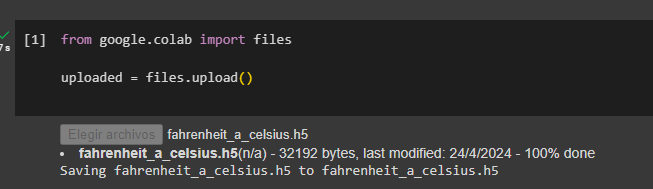
\includegraphics{Grados/img/Subir modelo.png}
\caption{image.png}
\end{figure}

    Creamos la carpeta de salida e instalamos tensorflowjs

    \begin{figure}
\centering
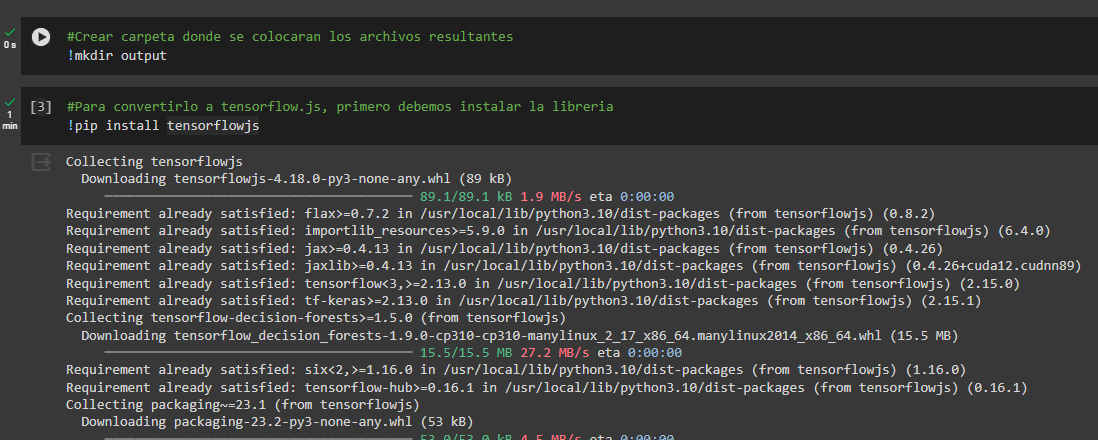
\includegraphics{Grados/img/crear carpeta y instalar tensorflowjs.png}
\caption{image.png}
\end{figure}

    Con tensorflowjs generamos los archivos json y bin necesarios para
mostrar los resultados en la web

    \begin{figure}
\centering
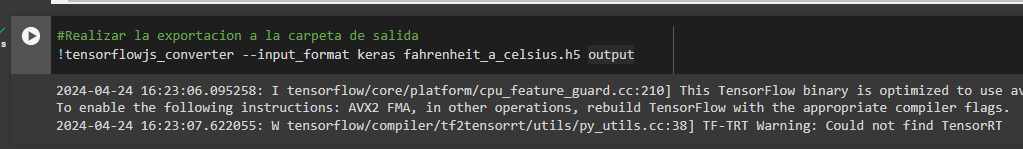
\includegraphics{Grados/img/generar json.png}
\caption{image.png}
\end{figure}

    Aqui podemos ver los archivos generados, ahora los descargamos en la
carpeta donde tenemos guardado la pagina web

    \begin{figure}
\centering
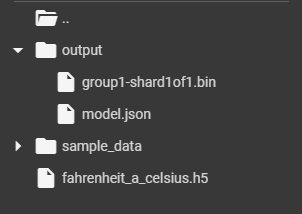
\includegraphics{Grados/img/archivos generados.png}
\caption{image.png}
\end{figure}

    Abrimos el servidor en la carpeta donde tenemos guardado la pagina web

    \begin{figure}
\centering
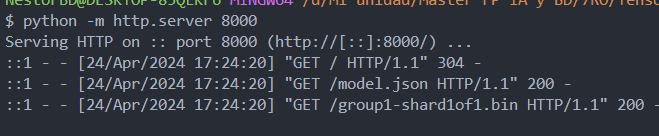
\includegraphics{Grados/img/abrir servidor.png}
\caption{image.png}
\end{figure}

    Y por ultimo abrimos el siguiente \href{http://localhost:8000}{link} en
el navegador

    \begin{figure}
\centering

\includegraphics{Grados/img/Fahreanheit a Celsius WEB.png}
\caption{image.png}
\end{figure}

    \section{Clasificación de flores}\label{clasificaciuxf3n-de-flores}

    \begin{tcolorbox}[breakable, size=fbox, boxrule=1pt, pad at break*=1mm,colback=white, colframe=black]
\prompt{In}{incolor}{1}{\boxspacing}
\begin{Verbatim}[commandchars=\\\{\}]
\PY{k+kn}{import} \PY{n+nn}{tensorflow} \PY{k}{as} \PY{n+nn}{tf}
\PY{k+kn}{from} \PY{n+nn}{tensorflow}\PY{n+nn}{.}\PY{n+nn}{keras}\PY{n+nn}{.}\PY{n+nn}{preprocessing}\PY{n+nn}{.}\PY{n+nn}{image} \PY{k+kn}{import} \PY{n}{ImageDataGenerator}
\PY{k+kn}{import} \PY{n+nn}{os}
\PY{k+kn}{import} \PY{n+nn}{numpy} \PY{k}{as} \PY{n+nn}{np}
\PY{k+kn}{import} \PY{n+nn}{matplotlib}\PY{n+nn}{.}\PY{n+nn}{pyplot} \PY{k}{as} \PY{n+nn}{plt}
\PY{k+kn}{import} \PY{n+nn}{splitfolders}
\PY{k+kn}{import} \PY{n+nn}{cv2}
\PY{k+kn}{import} \PY{n+nn}{seaborn} \PY{k}{as} \PY{n+nn}{sns}
\PY{k+kn}{from} \PY{n+nn}{sklearn}\PY{n+nn}{.}\PY{n+nn}{metrics} \PY{k+kn}{import} \PY{n}{confusion\PYZus{}matrix}\PY{p}{,} \PY{n}{classification\PYZus{}report}
\end{Verbatim}
\end{tcolorbox}

\begin{tcolorbox}[breakable, size=fbox, boxrule=1pt, pad at break*=1mm,colback=cellbackground, colframe=cellborder]
    \prompt{Out}{outcolor}{1}{\boxspacing} 
    \begin{Verbatim}[commandchars=\\\{\}]
WARNING:tensorflow:From c:\textbackslash{}Users\textbackslash{}NestorBD\textbackslash{}anaconda3\textbackslash{}Lib\textbackslash{}site-
packages\textbackslash{}keras\textbackslash{}src\textbackslash{}losses.py:2976: The name
tf.losses.sparse\_softmax\_cross\_entropy is deprecated. Please use
tf.compat.v1.losses.sparse\_softmax\_cross\_entropy instead.

    \end{Verbatim}
\end{tcolorbox}

    Definimos la carpeta en donde se encuentran las imagenes con las que
vamos a entrenar el modelo

    \begin{tcolorbox}[breakable, size=fbox, boxrule=1pt, pad at break*=1mm,colback=white, colframe=black]
\prompt{In}{incolor}{2}{\boxspacing}
\begin{Verbatim}[commandchars=\\\{\}]
\PY{n}{original\PYZus{}path} \PY{o}{=} \PY{l+s+s2}{\PYZdq{}}\PY{l+s+s2}{Flores/flowers}\PY{l+s+s2}{\PYZdq{}}
\PY{n+nb}{print}\PY{p}{(}\PY{n}{os}\PY{o}{.}\PY{n}{listdir}\PY{p}{(}\PY{n}{original\PYZus{}path}\PY{p}{)}\PY{p}{)}
\end{Verbatim}
\end{tcolorbox}

\begin{tcolorbox}[breakable, size=fbox, boxrule=1pt, pad at break*=1mm,colback=cellbackground, colframe=cellborder]
    \prompt{Out}{outcolor}{2}{\boxspacing} 
    \begin{Verbatim}[commandchars=\\\{\}]
['daisy', 'dandelion', 'rose', 'sunflower', 'tulip']
    \end{Verbatim}
\end{tcolorbox}

    Creamos un MAP con las especies de flores que tenemos para entrenar y
definimos el tamaño de las imagenes

    \begin{tcolorbox}[breakable, size=fbox, boxrule=1pt, pad at break*=1mm,colback=white, colframe=black]
\prompt{In}{incolor}{3}{\boxspacing}
\begin{Verbatim}[commandchars=\\\{\}]
\PY{n}{MAP\PYZus{}FLOWERS} \PY{o}{=} \PY{p}{\PYZob{}}
    \PY{l+m+mi}{0}\PY{p}{:} \PY{l+s+s1}{\PYZsq{}}\PY{l+s+s1}{daisy}\PY{l+s+s1}{\PYZsq{}}\PY{p}{,} \PY{l+m+mi}{1}\PY{p}{:} \PY{l+s+s1}{\PYZsq{}}\PY{l+s+s1}{dandelion}\PY{l+s+s1}{\PYZsq{}}\PY{p}{,} \PY{l+m+mi}{2}\PY{p}{:} \PY{l+s+s1}{\PYZsq{}}\PY{l+s+s1}{rose}\PY{l+s+s1}{\PYZsq{}}\PY{p}{,} 
    \PY{l+m+mi}{3}\PY{p}{:} \PY{l+s+s1}{\PYZsq{}}\PY{l+s+s1}{sunflower}\PY{l+s+s1}{\PYZsq{}}\PY{p}{,} \PY{l+m+mi}{4}\PY{p}{:} \PY{l+s+s1}{\PYZsq{}}\PY{l+s+s1}{tulip}\PY{l+s+s1}{\PYZsq{}}
\PY{p}{\PYZcb{}}

\PY{c+c1}{\PYZsh{} Vamos a standarizar todas las imágenes a tamaño 128x128}
\PY{n}{IMG\PYZus{}SIZE} \PY{o}{=} \PY{l+m+mi}{128}
\end{Verbatim}
\end{tcolorbox}

    Dividimos los archivos en tres conjuntos entrenamiento, validación y
pruebas

    \begin{tcolorbox}[breakable, size=fbox, boxrule=1pt, pad at break*=1mm,colback=white, colframe=black]
\prompt{In}{incolor}{4}{\boxspacing}
\begin{Verbatim}[commandchars=\\\{\}]
\PY{n}{splitfolders}\PY{o}{.}\PY{n}{ratio}\PY{p}{(}\PY{l+s+s1}{\PYZsq{}}\PY{l+s+s1}{Flores/flowers}\PY{l+s+s1}{\PYZsq{}}\PY{p}{,}\PY{n}{seed}\PY{o}{=}\PY{l+m+mi}{1337}\PY{p}{,} \PY{n}{output}\PY{o}{=}\PY{l+s+s2}{\PYZdq{}}\PY{l+s+s2}{Flores/Flowers\PYZhy{}Splitted}\PY{l+s+s2}{\PYZdq{}}\PY{p}{,} \PY{n}{ratio}\PY{o}{=}\PY{p}{(}\PY{l+m+mf}{0.6}\PY{p}{,} \PY{l+m+mf}{0.2}\PY{p}{,} \PY{l+m+mf}{0.2}\PY{p}{)}\PY{p}{)}
\end{Verbatim}
\end{tcolorbox}

\begin{tcolorbox}[breakable, size=fbox, boxrule=1pt, pad at break*=1mm,colback=cellbackground, colframe=cellborder]
    \prompt{Out}{outcolor}{4}{\boxspacing} 
    \begin{Verbatim}[commandchars=\\\{\}]
Copying files: 2131 files [00:33, 60.96 files/s]
    \end{Verbatim}
\end{tcolorbox}

    Creamos las funciones para cargar las imagenes

    \begin{tcolorbox}[breakable, size=fbox, boxrule=1pt, pad at break*=1mm,colback=white, colframe=black]
\prompt{In}{incolor}{6}{\boxspacing}
\begin{Verbatim}[commandchars=\\\{\}]
\PY{k}{def} \PY{n+nf}{load\PYZus{}train\PYZus{}set}\PY{p}{(}\PY{n}{dirname}\PY{p}{,} \PY{n}{map\PYZus{}pieces}\PY{p}{,} \PY{n}{verbose}\PY{o}{=}\PY{k+kc}{True}\PY{p}{)}\PY{p}{:}
\PY{+w}{    }\PY{l+s+sd}{\PYZdq{}\PYZdq{}\PYZdq{}Esta función carga los datos de training en imágenes.}

\PY{l+s+sd}{    Como las imágenes tienen tamaños distintas, utilizamos la librería opencv}
\PY{l+s+sd}{    para hacer un resize y adaptarlas todas a tamaño IMG\PYZus{}SIZE x IMG\PYZus{}SIZE.}

\PY{l+s+sd}{    Args:}
\PY{l+s+sd}{        dirname: directorio completo del que leer los datos}
\PY{l+s+sd}{        map\PYZus{}pieces: variable de mapeo entre labels y piezas}
\PY{l+s+sd}{        verbose: si es True, muestra información de las imágenes cargadas}

\PY{l+s+sd}{    Returns:}
\PY{l+s+sd}{        X, y: X es un array con todas las imágenes cargadas con tamaño}
\PY{l+s+sd}{                IMG\PYZus{}SIZE x IMG\PYZus{}SIZE}
\PY{l+s+sd}{              y es un array con las labels de correspondientes a cada imagen}
\PY{l+s+sd}{    \PYZdq{}\PYZdq{}\PYZdq{}}
    \PY{n}{X\PYZus{}train} \PY{o}{=} \PY{p}{[}\PY{p}{]}
    \PY{n}{y\PYZus{}train} \PY{o}{=} \PY{p}{[}\PY{p}{]}
    \PY{k}{for} \PY{n}{label}\PY{p}{,} \PY{n}{piece} \PY{o+ow}{in} \PY{n}{map\PYZus{}pieces}\PY{o}{.}\PY{n}{items}\PY{p}{(}\PY{p}{)}\PY{p}{:}
        \PY{n}{files} \PY{o}{=} \PY{n}{os}\PY{o}{.}\PY{n}{listdir}\PY{p}{(}\PY{n}{os}\PY{o}{.}\PY{n}{path}\PY{o}{.}\PY{n}{join}\PY{p}{(}\PY{n}{dirname}\PY{p}{,} \PY{n}{piece}\PY{p}{)}\PY{p}{)}
        \PY{n}{images} \PY{o}{=} \PY{p}{[}\PY{n}{file} \PY{k}{for} \PY{n}{file} \PY{o+ow}{in} \PY{n}{files} \PY{k}{if} \PY{p}{(}\PY{n}{file}\PY{o}{.}\PY{n}{endswith}\PY{p}{(}\PY{l+s+s2}{\PYZdq{}}\PY{l+s+s2}{jpg}\PY{l+s+s2}{\PYZdq{}}\PY{p}{)} \PY{o+ow}{or} \PY{n}{file}\PY{o}{.}\PY{n}{endswith}\PY{p}{(}\PY{l+s+s2}{\PYZdq{}}\PY{l+s+s2}{png}\PY{l+s+s2}{\PYZdq{}}\PY{p}{)} \PY{o+ow}{or} \PY{n}{file}\PY{o}{.}\PY{n}{endswith}\PY{p}{(}\PY{l+s+s2}{\PYZdq{}}\PY{l+s+s2}{jpeg}\PY{l+s+s2}{\PYZdq{}}\PY{p}{)} \PY{o+ow}{or} \PY{n}{file}\PY{o}{.}\PY{n}{endswith}\PY{p}{(}\PY{l+s+s2}{\PYZdq{}}\PY{l+s+s2}{JPG}\PY{l+s+s2}{\PYZdq{}}\PY{p}{)}\PY{p}{)}\PY{p}{]}
        \PY{k}{if} \PY{n}{verbose}\PY{p}{:}
          \PY{n+nb}{print}\PY{p}{(}\PY{l+s+s2}{\PYZdq{}}\PY{l+s+s2}{Leyendo }\PY{l+s+si}{\PYZob{}\PYZcb{}}\PY{l+s+s2}{ imágenes encontradas de }\PY{l+s+si}{\PYZob{}\PYZcb{}}\PY{l+s+s2}{\PYZdq{}}\PY{o}{.}\PY{n}{format}\PY{p}{(}\PY{n+nb}{len}\PY{p}{(}\PY{n}{images}\PY{p}{)}\PY{p}{,} \PY{n}{piece}\PY{p}{)}\PY{p}{)}
        \PY{k}{for} \PY{n}{image\PYZus{}name} \PY{o+ow}{in} \PY{n}{images}\PY{p}{:}
            \PY{n}{image} \PY{o}{=} \PY{n}{cv2}\PY{o}{.}\PY{n}{imread}\PY{p}{(}\PY{n}{os}\PY{o}{.}\PY{n}{path}\PY{o}{.}\PY{n}{join}\PY{p}{(}\PY{n}{dirname}\PY{p}{,} \PY{n}{piece}\PY{p}{,} \PY{n}{image\PYZus{}name}\PY{p}{)}\PY{p}{)}
            \PY{n}{X\PYZus{}train}\PY{o}{.}\PY{n}{append}\PY{p}{(}\PY{n}{cv2}\PY{o}{.}\PY{n}{resize}\PY{p}{(}\PY{n}{image}\PY{p}{,}\PY{p}{(}\PY{n}{IMG\PYZus{}SIZE}\PY{p}{,} \PY{n}{IMG\PYZus{}SIZE}\PY{p}{)}\PY{p}{)}\PY{p}{)}
            \PY{n}{y\PYZus{}train}\PY{o}{.}\PY{n}{append}\PY{p}{(}\PY{n}{label}\PY{p}{)}
    \PY{k}{return} \PY{n}{np}\PY{o}{.}\PY{n}{array}\PY{p}{(}\PY{n}{X\PYZus{}train}\PY{p}{)}\PY{p}{,} \PY{n}{np}\PY{o}{.}\PY{n}{array}\PY{p}{(}\PY{n}{y\PYZus{}train}\PY{p}{)}
\end{Verbatim}
\end{tcolorbox}

    \begin{tcolorbox}[breakable, size=fbox, boxrule=1pt, pad at break*=1mm,colback=white, colframe=black]
\prompt{In}{incolor}{7}{\boxspacing}
\begin{Verbatim}[commandchars=\\\{\}]
\PY{k}{def} \PY{n+nf}{load\PYZus{}test\PYZus{}or\PYZus{}val\PYZus{}set}\PY{p}{(}\PY{n}{dirname}\PY{p}{,} \PY{n}{map\PYZus{}pieces}\PY{p}{,} \PY{n}{verbose}\PY{o}{=}\PY{k+kc}{True}\PY{p}{,} \PY{n}{isTest}\PY{o}{=}\PY{k+kc}{True}\PY{p}{)}\PY{p}{:}
\PY{+w}{    }\PY{l+s+sd}{\PYZdq{}\PYZdq{}\PYZdq{}Esta función funciona de manera equivalente a la función load\PYZus{}train\PYZus{}set}
\PY{l+s+sd}{    pero cargando los datos de test.\PYZdq{}\PYZdq{}\PYZdq{}}
    \PY{n}{X\PYZus{}test} \PY{o}{=} \PY{p}{[}\PY{p}{]}
    \PY{n}{y\PYZus{}test} \PY{o}{=} \PY{p}{[}\PY{p}{]}
    \PY{k}{for} \PY{n}{label}\PY{p}{,} \PY{n}{piece} \PY{o+ow}{in} \PY{n}{map\PYZus{}pieces}\PY{o}{.}\PY{n}{items}\PY{p}{(}\PY{p}{)}\PY{p}{:}
        \PY{n}{files} \PY{o}{=} \PY{n}{os}\PY{o}{.}\PY{n}{listdir}\PY{p}{(}\PY{n}{os}\PY{o}{.}\PY{n}{path}\PY{o}{.}\PY{n}{join}\PY{p}{(}\PY{n}{dirname}\PY{p}{,} \PY{n}{piece}\PY{p}{)}\PY{p}{)}
        \PY{n}{images} \PY{o}{=} \PY{p}{[}\PY{n}{file} \PY{k}{for} \PY{n}{file} \PY{o+ow}{in} \PY{n}{files} \PY{k}{if} \PY{p}{(}\PY{n}{file}\PY{o}{.}\PY{n}{endswith}\PY{p}{(}\PY{l+s+s2}{\PYZdq{}}\PY{l+s+s2}{jpg}\PY{l+s+s2}{\PYZdq{}}\PY{p}{)} \PY{o+ow}{or} \PY{n}{file}\PY{o}{.}\PY{n}{endswith}\PY{p}{(}\PY{l+s+s2}{\PYZdq{}}\PY{l+s+s2}{png}\PY{l+s+s2}{\PYZdq{}}\PY{p}{)} \PY{o+ow}{or} \PY{n}{file}\PY{o}{.}\PY{n}{endswith}\PY{p}{(}\PY{l+s+s2}{\PYZdq{}}\PY{l+s+s2}{jpeg}\PY{l+s+s2}{\PYZdq{}}\PY{p}{)} \PY{o+ow}{or} \PY{n}{file}\PY{o}{.}\PY{n}{endswith}\PY{p}{(}\PY{l+s+s2}{\PYZdq{}}\PY{l+s+s2}{JPG}\PY{l+s+s2}{\PYZdq{}}\PY{p}{)}\PY{p}{)}\PY{p}{]}
        \PY{k}{for} \PY{n}{image\PYZus{}name} \PY{o+ow}{in} \PY{n}{images}\PY{p}{:}
            \PY{n}{image} \PY{o}{=} \PY{n}{cv2}\PY{o}{.}\PY{n}{imread}\PY{p}{(}\PY{n}{os}\PY{o}{.}\PY{n}{path}\PY{o}{.}\PY{n}{join}\PY{p}{(}\PY{n}{dirname}\PY{p}{,} \PY{n}{piece}\PY{p}{,} \PY{n}{image\PYZus{}name}\PY{p}{)}\PY{p}{)}
            \PY{n}{X\PYZus{}test}\PY{o}{.}\PY{n}{append}\PY{p}{(}\PY{n}{cv2}\PY{o}{.}\PY{n}{resize}\PY{p}{(}\PY{n}{image}\PY{p}{,}\PY{p}{(}\PY{n}{IMG\PYZus{}SIZE}\PY{p}{,} \PY{n}{IMG\PYZus{}SIZE}\PY{p}{)}\PY{p}{)}\PY{p}{)}
            \PY{n}{y\PYZus{}test}\PY{o}{.}\PY{n}{append}\PY{p}{(}\PY{n}{label}\PY{p}{)}
    \PY{k}{if} \PY{n}{verbose}\PY{p}{:}
        \PY{k}{if} \PY{n}{isTest}\PY{p}{:}
            \PY{n+nb}{print}\PY{p}{(}\PY{l+s+s2}{\PYZdq{}}\PY{l+s+s2}{Leídas }\PY{l+s+si}{\PYZob{}\PYZcb{}}\PY{l+s+s2}{ imágenes de test}\PY{l+s+s2}{\PYZdq{}}\PY{o}{.}\PY{n}{format}\PY{p}{(}\PY{n+nb}{len}\PY{p}{(}\PY{n}{X\PYZus{}test}\PY{p}{)}\PY{p}{)}\PY{p}{)}
        \PY{k}{else}\PY{p}{:}
            \PY{n+nb}{print}\PY{p}{(}\PY{l+s+s2}{\PYZdq{}}\PY{l+s+s2}{Leídas }\PY{l+s+si}{\PYZob{}\PYZcb{}}\PY{l+s+s2}{ imágenes de val}\PY{l+s+s2}{\PYZdq{}}\PY{o}{.}\PY{n}{format}\PY{p}{(}\PY{n+nb}{len}\PY{p}{(}\PY{n}{X\PYZus{}test}\PY{p}{)}\PY{p}{)}\PY{p}{)}
    \PY{k}{return} \PY{n}{np}\PY{o}{.}\PY{n}{array}\PY{p}{(}\PY{n}{X\PYZus{}test}\PY{p}{)}\PY{p}{,} \PY{n}{np}\PY{o}{.}\PY{n}{array}\PY{p}{(}\PY{n}{y\PYZus{}test}\PY{p}{)}
\end{Verbatim}
\end{tcolorbox}

    Cargamos los datos.

    \begin{tcolorbox}[breakable, size=fbox, boxrule=1pt, pad at break*=1mm,colback=white, colframe=black]
\prompt{In}{incolor}{10}{\boxspacing}
\begin{Verbatim}[commandchars=\\\{\}]
\PY{n}{DATASET\PYZus{}TRAIN\PYZus{}PATH} \PY{o}{=} \PY{l+s+s2}{\PYZdq{}}\PY{l+s+s2}{Flores/Flowers\PYZhy{}Splitted/train}\PY{l+s+s2}{\PYZdq{}}
\PY{n}{DATASET\PYZus{}VAL\PYZus{}PATH} \PY{o}{=} \PY{l+s+s2}{\PYZdq{}}\PY{l+s+s2}{Flores/Flowers\PYZhy{}Splitted/val}\PY{l+s+s2}{\PYZdq{}}
\PY{n}{DATASET\PYZus{}TEST\PYZus{}PATH} \PY{o}{=} \PY{l+s+s2}{\PYZdq{}}\PY{l+s+s2}{Flores/Flowers\PYZhy{}Splitted/test}\PY{l+s+s2}{\PYZdq{}}

\PY{n}{X}\PY{p}{,} \PY{n}{y} \PY{o}{=} \PY{n}{load\PYZus{}train\PYZus{}set}\PY{p}{(}\PY{n}{DATASET\PYZus{}TRAIN\PYZus{}PATH}\PY{p}{,} \PY{n}{MAP\PYZus{}FLOWERS}\PY{p}{)}
\PY{n}{X\PYZus{}v}\PY{p}{,} \PY{n}{y\PYZus{}v} \PY{o}{=} \PY{n}{load\PYZus{}test\PYZus{}or\PYZus{}val\PYZus{}set}\PY{p}{(}\PY{n}{DATASET\PYZus{}TEST\PYZus{}PATH}\PY{p}{,} \PY{n}{MAP\PYZus{}FLOWERS}\PY{p}{,} \PY{n}{isTest}\PY{o}{=}\PY{k+kc}{False}\PY{p}{)}
\PY{n}{X\PYZus{}t}\PY{p}{,} \PY{n}{y\PYZus{}t} \PY{o}{=} \PY{n}{load\PYZus{}test\PYZus{}or\PYZus{}val\PYZus{}set}\PY{p}{(}\PY{n}{DATASET\PYZus{}TEST\PYZus{}PATH}\PY{p}{,} \PY{n}{MAP\PYZus{}FLOWERS}\PY{p}{)}
\end{Verbatim}
\end{tcolorbox}

\begin{tcolorbox}[breakable, size=fbox, boxrule=1pt, pad at break*=1mm,colback=cellbackground, colframe=cellborder]
    \prompt{Out}{outcolor}{10}{\boxspacing} 
    \begin{Verbatim}[commandchars=\\\{\}]
Leyendo 300 imágenes encontradas de daisy
Leyendo 387 imágenes encontradas de dandelion
Leyendo 298 imágenes encontradas de rose
Leyendo 297 imágenes encontradas de sunflower
Leyendo 364 imágenes encontradas de tulip
Leídas 552 imágenes de val
Leídas 552 imágenes de test
    \end{Verbatim}
\end{tcolorbox}

    Aumentamos los datos de entrenamiento

    \begin{tcolorbox}[breakable, size=fbox, boxrule=1pt, pad at break*=1mm,colback=white, colframe=black]
\prompt{In}{incolor}{11}{\boxspacing}
\begin{Verbatim}[commandchars=\\\{\}]
\PY{c+c1}{\PYZsh{}Aumento de datos}
\PY{n}{image\PYZus{}gen\PYZus{}entrenamiento} \PY{o}{=} \PY{n}{ImageDataGenerator}\PY{p}{(}
      \PY{n}{rescale}\PY{o}{=}\PY{l+m+mf}{1.}\PY{o}{/}\PY{l+m+mi}{255}\PY{p}{,}
      \PY{n}{rotation\PYZus{}range}\PY{o}{=}\PY{l+m+mi}{40}\PY{p}{,}
      \PY{n}{width\PYZus{}shift\PYZus{}range}\PY{o}{=}\PY{l+m+mf}{0.2}\PY{p}{,}
      \PY{n}{height\PYZus{}shift\PYZus{}range}\PY{o}{=}\PY{l+m+mf}{0.2}\PY{p}{,}
      \PY{n}{shear\PYZus{}range}\PY{o}{=}\PY{l+m+mf}{0.2}\PY{p}{,}
      \PY{n}{zoom\PYZus{}range}\PY{o}{=}\PY{l+m+mf}{0.2}\PY{p}{,}
      \PY{n}{horizontal\PYZus{}flip}\PY{o}{=}\PY{k+kc}{True}\PY{p}{,}
      \PY{n}{fill\PYZus{}mode}\PY{o}{=}\PY{l+s+s1}{\PYZsq{}}\PY{l+s+s1}{nearest}\PY{l+s+s1}{\PYZsq{}}\PY{p}{)}
\end{Verbatim}
\end{tcolorbox}

    \begin{tcolorbox}[breakable, size=fbox, boxrule=1pt, pad at break*=1mm,colback=white, colframe=black]
\prompt{In}{incolor}{12}{\boxspacing}
\begin{Verbatim}[commandchars=\\\{\}]
\PY{c+c1}{\PYZsh{}Generacion de datos de entrenamiento FTW}
\PY{n}{data\PYZus{}gen\PYZus{}entrenamiento} \PY{o}{=} \PY{n}{image\PYZus{}gen\PYZus{}entrenamiento}\PY{o}{.}\PY{n}{flow\PYZus{}from\PYZus{}directory}\PY{p}{(}\PY{n}{batch\PYZus{}size}\PY{o}{=}\PY{l+m+mi}{100}\PY{p}{,}
                                                     \PY{n}{directory}\PY{o}{=}\PY{l+s+s2}{\PYZdq{}}\PY{l+s+s2}{Flores/Flowers\PYZhy{}Splitted/train}\PY{l+s+s2}{\PYZdq{}}\PY{p}{,}
                                                     \PY{n}{shuffle}\PY{o}{=}\PY{k+kc}{True}\PY{p}{,}
                                                     \PY{n}{target\PYZus{}size}\PY{o}{=}\PY{p}{(}\PY{n}{IMG\PYZus{}SIZE}\PY{p}{,}\PY{n}{IMG\PYZus{}SIZE}\PY{p}{)}\PY{p}{,}
                                                     \PY{n}{class\PYZus{}mode}\PY{o}{=}\PY{l+s+s1}{\PYZsq{}}\PY{l+s+s1}{categorical}\PY{l+s+s1}{\PYZsq{}}\PY{p}{)}
\end{Verbatim}
\end{tcolorbox}

\begin{tcolorbox}[breakable, size=fbox, boxrule=1pt, pad at break*=1mm,colback=cellbackground, colframe=cellborder]
    \prompt{Out}{outcolor}{12}{\boxspacing} 
    \begin{Verbatim}[commandchars=\\\{\}]
Found 1646 images belonging to 5 classes.
    \end{Verbatim}
\end{tcolorbox}

    Rescalamos los datos de validación para que sean iguales a los de
entrenamiento.

    \begin{tcolorbox}[breakable, size=fbox, boxrule=1pt, pad at break*=1mm,colback=white, colframe=black]
\prompt{In}{incolor}{13}{\boxspacing}
\begin{Verbatim}[commandchars=\\\{\}]
\PY{c+c1}{\PYZsh{}Generacion de datos de validacion}
\PY{n}{image\PYZus{}gen\PYZus{}val} \PY{o}{=} \PY{n}{ImageDataGenerator}\PY{p}{(}\PY{n}{rescale}\PY{o}{=}\PY{l+m+mf}{1.}\PY{o}{/}\PY{l+m+mi}{255}\PY{p}{)}

\PY{n}{data\PYZus{}gen\PYZus{}validacion} \PY{o}{=} \PY{n}{image\PYZus{}gen\PYZus{}val}\PY{o}{.}\PY{n}{flow\PYZus{}from\PYZus{}directory}\PY{p}{(}\PY{n}{batch\PYZus{}size}\PY{o}{=}\PY{l+m+mi}{100}\PY{p}{,}
                                                 \PY{n}{directory}\PY{o}{=}\PY{l+s+s2}{\PYZdq{}}\PY{l+s+s2}{Flores/Flowers\PYZhy{}Splitted/val}\PY{l+s+s2}{\PYZdq{}}\PY{p}{,}
                                                 \PY{n}{target\PYZus{}size}\PY{o}{=}\PY{p}{(}\PY{n}{IMG\PYZus{}SIZE}\PY{p}{,} \PY{n}{IMG\PYZus{}SIZE}\PY{p}{)}\PY{p}{,}
                                                 \PY{n}{class\PYZus{}mode}\PY{o}{=}\PY{l+s+s1}{\PYZsq{}}\PY{l+s+s1}{categorical}\PY{l+s+s1}{\PYZsq{}}\PY{p}{)}
\end{Verbatim}
\end{tcolorbox}

\begin{tcolorbox}[breakable, size=fbox, boxrule=1pt, pad at break*=1mm,colback=cellbackground, colframe=cellborder]
    \prompt{Out}{outcolor}{13}{\boxspacing} 
    \begin{Verbatim}[commandchars=\\\{\}]
Found 548 images belonging to 5 classes.
    \end{Verbatim}
\end{tcolorbox}

    Craemos el modelo muy sencillo, tal cual esta en el video,solo cambiando
los datos de salida, sino puede dar fallos.

    \begin{tcolorbox}[breakable, size=fbox, boxrule=1pt, pad at break*=1mm,colback=white, colframe=black]
\prompt{In}{incolor}{42}{\boxspacing}
\begin{Verbatim}[commandchars=\\\{\}]
\PY{n}{modelo} \PY{o}{=} \PY{n}{tf}\PY{o}{.}\PY{n}{keras}\PY{o}{.}\PY{n}{models}\PY{o}{.}\PY{n}{Sequential}\PY{p}{(}\PY{p}{[}
    \PY{n}{tf}\PY{o}{.}\PY{n}{keras}\PY{o}{.}\PY{n}{layers}\PY{o}{.}\PY{n}{Conv2D}\PY{p}{(}\PY{l+m+mi}{32}\PY{p}{,} \PY{p}{(}\PY{l+m+mi}{3}\PY{p}{,}\PY{l+m+mi}{3}\PY{p}{)}\PY{p}{,} \PY{n}{activation}\PY{o}{=}\PY{l+s+s1}{\PYZsq{}}\PY{l+s+s1}{relu}\PY{l+s+s1}{\PYZsq{}}\PY{p}{,} \PY{n}{input\PYZus{}shape}\PY{o}{=}\PY{p}{(}\PY{n}{IMG\PYZus{}SIZE}\PY{p}{,} \PY{n}{IMG\PYZus{}SIZE}\PY{p}{,} \PY{l+m+mi}{3}\PY{p}{)}\PY{p}{)}\PY{p}{,}
    \PY{n}{tf}\PY{o}{.}\PY{n}{keras}\PY{o}{.}\PY{n}{layers}\PY{o}{.}\PY{n}{MaxPooling2D}\PY{p}{(}\PY{l+m+mi}{2}\PY{p}{,} \PY{l+m+mi}{2}\PY{p}{)}\PY{p}{,}

    \PY{n}{tf}\PY{o}{.}\PY{n}{keras}\PY{o}{.}\PY{n}{layers}\PY{o}{.}\PY{n}{Conv2D}\PY{p}{(}\PY{l+m+mi}{64}\PY{p}{,} \PY{p}{(}\PY{l+m+mi}{3}\PY{p}{,}\PY{l+m+mi}{3}\PY{p}{)}\PY{p}{,} \PY{n}{activation}\PY{o}{=}\PY{l+s+s1}{\PYZsq{}}\PY{l+s+s1}{relu}\PY{l+s+s1}{\PYZsq{}}\PY{p}{)}\PY{p}{,}
    \PY{n}{tf}\PY{o}{.}\PY{n}{keras}\PY{o}{.}\PY{n}{layers}\PY{o}{.}\PY{n}{MaxPooling2D}\PY{p}{(}\PY{l+m+mi}{2}\PY{p}{,}\PY{l+m+mi}{2}\PY{p}{)}\PY{p}{,}

    \PY{n}{tf}\PY{o}{.}\PY{n}{keras}\PY{o}{.}\PY{n}{layers}\PY{o}{.}\PY{n}{Conv2D}\PY{p}{(}\PY{l+m+mi}{128}\PY{p}{,} \PY{p}{(}\PY{l+m+mi}{3}\PY{p}{,}\PY{l+m+mi}{3}\PY{p}{)}\PY{p}{,} \PY{n}{activation}\PY{o}{=}\PY{l+s+s1}{\PYZsq{}}\PY{l+s+s1}{relu}\PY{l+s+s1}{\PYZsq{}}\PY{p}{)}\PY{p}{,}
    \PY{n}{tf}\PY{o}{.}\PY{n}{keras}\PY{o}{.}\PY{n}{layers}\PY{o}{.}\PY{n}{MaxPooling2D}\PY{p}{(}\PY{l+m+mi}{2}\PY{p}{,}\PY{l+m+mi}{2}\PY{p}{)}\PY{p}{,}

    \PY{n}{tf}\PY{o}{.}\PY{n}{keras}\PY{o}{.}\PY{n}{layers}\PY{o}{.}\PY{n}{Conv2D}\PY{p}{(}\PY{l+m+mi}{128}\PY{p}{,} \PY{p}{(}\PY{l+m+mi}{3}\PY{p}{,}\PY{l+m+mi}{3}\PY{p}{)}\PY{p}{,} \PY{n}{activation}\PY{o}{=}\PY{l+s+s1}{\PYZsq{}}\PY{l+s+s1}{relu}\PY{l+s+s1}{\PYZsq{}}\PY{p}{)}\PY{p}{,}
    \PY{n}{tf}\PY{o}{.}\PY{n}{keras}\PY{o}{.}\PY{n}{layers}\PY{o}{.}\PY{n}{MaxPooling2D}\PY{p}{(}\PY{l+m+mi}{2}\PY{p}{,}\PY{l+m+mi}{2}\PY{p}{)}\PY{p}{,}

    \PY{n}{tf}\PY{o}{.}\PY{n}{keras}\PY{o}{.}\PY{n}{layers}\PY{o}{.}\PY{n}{Dropout}\PY{p}{(}\PY{l+m+mf}{0.5}\PY{p}{)}\PY{p}{,}
    \PY{n}{tf}\PY{o}{.}\PY{n}{keras}\PY{o}{.}\PY{n}{layers}\PY{o}{.}\PY{n}{Flatten}\PY{p}{(}\PY{p}{)}\PY{p}{,}
    \PY{n}{tf}\PY{o}{.}\PY{n}{keras}\PY{o}{.}\PY{n}{layers}\PY{o}{.}\PY{n}{Dense}\PY{p}{(}\PY{l+m+mi}{512}\PY{p}{,} \PY{n}{activation}\PY{o}{=}\PY{l+s+s1}{\PYZsq{}}\PY{l+s+s1}{relu}\PY{l+s+s1}{\PYZsq{}}\PY{p}{)}\PY{p}{,}
    \PY{n}{tf}\PY{o}{.}\PY{n}{keras}\PY{o}{.}\PY{n}{layers}\PY{o}{.}\PY{n}{Dense}\PY{p}{(}\PY{l+m+mi}{5}\PY{p}{,} \PY{n}{activation}\PY{o}{=}\PY{l+s+s1}{\PYZsq{}}\PY{l+s+s1}{softmax}\PY{l+s+s1}{\PYZsq{}}\PY{p}{)}
\PY{p}{]}\PY{p}{)}
\end{Verbatim}
\end{tcolorbox}

    Compilación y entrenamiento

    \begin{tcolorbox}[breakable, size=fbox, boxrule=1pt, pad at break*=1mm,colback=white, colframe=black]
\prompt{In}{incolor}{43}{\boxspacing}
\begin{Verbatim}[commandchars=\\\{\}]
\PY{c+c1}{\PYZsh{}Compilación}
\PY{n}{modelo}\PY{o}{.}\PY{n}{compile}\PY{p}{(}\PY{n}{optimizer}\PY{o}{=}\PY{l+s+s1}{\PYZsq{}}\PY{l+s+s1}{adam}\PY{l+s+s1}{\PYZsq{}}\PY{p}{,}
              \PY{n}{loss}\PY{o}{=}\PY{n}{tf}\PY{o}{.}\PY{n}{keras}\PY{o}{.}\PY{n}{losses}\PY{o}{.}\PY{n}{CategoricalCrossentropy}\PY{p}{(}\PY{n}{from\PYZus{}logits}\PY{o}{=}\PY{k+kc}{True}\PY{p}{)}\PY{p}{,}
              \PY{n}{metrics}\PY{o}{=}\PY{p}{[}\PY{l+s+s1}{\PYZsq{}}\PY{l+s+s1}{accuracy}\PY{l+s+s1}{\PYZsq{}}\PY{p}{]}\PY{p}{)}

\PY{c+c1}{\PYZsh{}Entrenar la red. Toma un buen rato! Ve por un café ;)}
\PY{c+c1}{\PYZsh{}Oye suscribete al canal!}
\PY{n+nb}{print}\PY{p}{(}\PY{l+s+s2}{\PYZdq{}}\PY{l+s+s2}{Entrenando modelo...}\PY{l+s+s2}{\PYZdq{}}\PY{p}{)}\PY{p}{;}
\PY{n}{epocas}\PY{o}{=}\PY{l+m+mi}{60}
\PY{n}{history} \PY{o}{=} \PY{n}{modelo}\PY{o}{.}\PY{n}{fit}\PY{p}{(}
    \PY{n}{data\PYZus{}gen\PYZus{}entrenamiento}\PY{p}{,}
    \PY{n}{steps\PYZus{}per\PYZus{}epoch}\PY{o}{=}\PY{n+nb}{int}\PY{p}{(}\PY{n}{np}\PY{o}{.}\PY{n}{ceil}\PY{p}{(}\PY{n+nb}{len}\PY{p}{(}\PY{n}{X}\PY{p}{)} \PY{o}{/} \PY{n+nb}{float}\PY{p}{(}\PY{l+m+mi}{100}\PY{p}{)}\PY{p}{)}\PY{p}{)}\PY{p}{,}
    \PY{n}{epochs}\PY{o}{=}\PY{n}{epocas}\PY{p}{,}
    \PY{n}{validation\PYZus{}data}\PY{o}{=}\PY{n}{data\PYZus{}gen\PYZus{}validacion}\PY{p}{,}
    \PY{n}{validation\PYZus{}steps}\PY{o}{=}\PY{n+nb}{int}\PY{p}{(}\PY{n}{np}\PY{o}{.}\PY{n}{ceil}\PY{p}{(}\PY{n+nb}{len}\PY{p}{(}\PY{n}{X\PYZus{}v}\PY{p}{)} \PY{o}{/} \PY{n+nb}{float}\PY{p}{(}\PY{l+m+mi}{100}\PY{p}{)}\PY{p}{)}\PY{p}{)}
\PY{p}{)}

\PY{n+nb}{print}\PY{p}{(}\PY{l+s+s2}{\PYZdq{}}\PY{l+s+s2}{Modelo entrenado!}\PY{l+s+s2}{\PYZdq{}}\PY{p}{)}\PY{p}{;}
\end{Verbatim}
\end{tcolorbox}

\begin{tcolorbox}[breakable, size=fbox, boxrule=1pt, pad at break*=1mm,colback=cellbackground, colframe=cellborder]
    \prompt{Out}{outcolor}{43}{\boxspacing} 
    \begin{Verbatim}[commandchars=\\\{\}]
Entrenando modelo{\ldots}
Epoch 1/60
    \end{Verbatim}

    \begin{Verbatim}[commandchars=\\\{\}]
c:\textbackslash{}Users\textbackslash{}NestorBD\textbackslash{}anaconda3\textbackslash{}Lib\textbackslash{}site-packages\textbackslash{}keras\textbackslash{}src\textbackslash{}backend.py:5575:
UserWarning: "`categorical\_crossentropy` received `from\_logits=True`, but the
`output` argument was produced by a Softmax activation and thus does not
represent logits. Was this intended?
  output, from\_logits = \_get\_logits(
    \end{Verbatim}

    \begin{Verbatim}[commandchars=\\\{\}]
17/17 \textcolor{ansi-green}{-----------------------} 37s 2s/step - loss: 1.5333 - accuracy:
0.2807 - val\_loss: 1.2777 - val\_accuracy: 0.4507
Epoch 2/60
17/17 \textcolor{ansi-green}{-----------------------} 33s 2s/step - loss: 1.2364 - accuracy:
0.4459 - val\_loss: 1.2061 - val\_accuracy: 0.4653
Epoch 3/60
17/17 \textcolor{ansi-green}{-----------------------} 33s 2s/step - loss: 1.1604 - accuracy:
0.5200 - val\_loss: 1.1896 - val\_accuracy: 0.5182
Epoch 4/60
17/17 \textcolor{ansi-green}{-----------------------} 33s 2s/step - loss: 1.0834 - accuracy:
0.5462 - val\_loss: 1.0571 - val\_accuracy: 0.5803
Epoch 5/60
17/17 \textcolor{ansi-green}{-----------------------} 34s 2s/step - loss: 1.1077 - accuracy:
0.5504 - val\_loss: 1.0573 - val\_accuracy: 0.5584
\text{........}
Epoch 55/60
17/17 \textcolor{ansi-green}{-----------------------} 41s 2s/step - loss: 0.4568 - accuracy:
0.8311 - val\_loss: 0.6196 - val\_accuracy: 0.7810
Epoch 56/60
17/17 \textcolor{ansi-green}{-----------------------} 37s 2s/step - loss: 0.4396 - accuracy:
0.8262 - val\_loss: 0.6075 - val\_accuracy: 0.7938
Epoch 57/60
17/17 \textcolor{ansi-green}{-----------------------} 36s 2s/step - loss: 0.4176 - accuracy:
0.8469 - val\_loss: 0.6310 - val\_accuracy: 0.7701
Epoch 58/60
17/17 \textcolor{ansi-green}{-----------------------} 38s 2s/step - loss: 0.4362 - accuracy:
0.8275 - val\_loss: 0.7968 - val\_accuracy: 0.7810
Epoch 59/60
17/17 \textcolor{ansi-green}{-----------------------} 35s 2s/step - loss: 0.4145 - accuracy:
0.8451 - val\_loss: 0.6386 - val\_accuracy: 0.7719
Epoch 60/60
17/17 \textcolor{ansi-green}{-----------------------} 40s 2s/step - loss: 0.4002 - accuracy:
0.8481 - val\_loss: 0.6365 - val\_accuracy: 0.7847
Modelo entrenado!
    \end{Verbatim}
\end{tcolorbox}

    \begin{tcolorbox}[breakable, size=fbox, boxrule=1pt, pad at break*=1mm,colback=white, colframe=black]
\prompt{In}{incolor}{44}{\boxspacing}
\begin{Verbatim}[commandchars=\\\{\}]
\PY{k}{def} \PY{n+nf}{plot\PYZus{}acc}\PY{p}{(}\PY{n}{history}\PY{p}{,} \PY{n}{title}\PY{o}{=}\PY{l+s+s2}{\PYZdq{}}\PY{l+s+s2}{Model Accuracy}\PY{l+s+s2}{\PYZdq{}}\PY{p}{)}\PY{p}{:}
\PY{+w}{  }\PY{l+s+sd}{\PYZdq{}\PYZdq{}\PYZdq{}Imprime una gráfica mostrando la accuracy por epoch obtenida en un entrenamiento\PYZdq{}\PYZdq{}\PYZdq{}}
  \PY{n}{plt}\PY{o}{.}\PY{n}{plot}\PY{p}{(}\PY{n}{history}\PY{o}{.}\PY{n}{history}\PY{p}{[}\PY{l+s+s1}{\PYZsq{}}\PY{l+s+s1}{accuracy}\PY{l+s+s1}{\PYZsq{}}\PY{p}{]}\PY{p}{)}
  \PY{n}{plt}\PY{o}{.}\PY{n}{plot}\PY{p}{(}\PY{n}{history}\PY{o}{.}\PY{n}{history}\PY{p}{[}\PY{l+s+s1}{\PYZsq{}}\PY{l+s+s1}{val\PYZus{}accuracy}\PY{l+s+s1}{\PYZsq{}}\PY{p}{]}\PY{p}{)}
  \PY{n}{plt}\PY{o}{.}\PY{n}{title}\PY{p}{(}\PY{n}{title}\PY{p}{)}
  \PY{n}{plt}\PY{o}{.}\PY{n}{ylabel}\PY{p}{(}\PY{l+s+s1}{\PYZsq{}}\PY{l+s+s1}{Accuracy}\PY{l+s+s1}{\PYZsq{}}\PY{p}{)}
  \PY{n}{plt}\PY{o}{.}\PY{n}{xlabel}\PY{p}{(}\PY{l+s+s1}{\PYZsq{}}\PY{l+s+s1}{Epoch}\PY{l+s+s1}{\PYZsq{}}\PY{p}{)}
  \PY{n}{plt}\PY{o}{.}\PY{n}{legend}\PY{p}{(}\PY{p}{[}\PY{l+s+s1}{\PYZsq{}}\PY{l+s+s1}{Train}\PY{l+s+s1}{\PYZsq{}}\PY{p}{,} \PY{l+s+s1}{\PYZsq{}}\PY{l+s+s1}{Val}\PY{l+s+s1}{\PYZsq{}}\PY{p}{]}\PY{p}{,} \PY{n}{loc}\PY{o}{=}\PY{l+s+s1}{\PYZsq{}}\PY{l+s+s1}{upper left}\PY{l+s+s1}{\PYZsq{}}\PY{p}{)}
  \PY{n}{plt}\PY{o}{.}\PY{n}{show}\PY{p}{(}\PY{p}{)}
\PY{k}{def} \PY{n+nf}{plot\PYZus{}loss}\PY{p}{(}\PY{n}{history}\PY{p}{,} \PY{n}{title}\PY{o}{=}\PY{l+s+s2}{\PYZdq{}}\PY{l+s+s2}{Model Loss}\PY{l+s+s2}{\PYZdq{}}\PY{p}{)}\PY{p}{:}
\PY{+w}{  }\PY{l+s+sd}{\PYZdq{}\PYZdq{}\PYZdq{}Imprime una gráfica mostrando la pérdida por epoch obtenida en un entrenamiento\PYZdq{}\PYZdq{}\PYZdq{}}
  \PY{n}{plt}\PY{o}{.}\PY{n}{plot}\PY{p}{(}\PY{n}{history}\PY{o}{.}\PY{n}{history}\PY{p}{[}\PY{l+s+s1}{\PYZsq{}}\PY{l+s+s1}{loss}\PY{l+s+s1}{\PYZsq{}}\PY{p}{]}\PY{p}{)}
  \PY{n}{plt}\PY{o}{.}\PY{n}{plot}\PY{p}{(}\PY{n}{history}\PY{o}{.}\PY{n}{history}\PY{p}{[}\PY{l+s+s1}{\PYZsq{}}\PY{l+s+s1}{val\PYZus{}loss}\PY{l+s+s1}{\PYZsq{}}\PY{p}{]}\PY{p}{)}
  \PY{n}{plt}\PY{o}{.}\PY{n}{title}\PY{p}{(}\PY{n}{title}\PY{p}{)}
  \PY{n}{plt}\PY{o}{.}\PY{n}{ylabel}\PY{p}{(}\PY{l+s+s1}{\PYZsq{}}\PY{l+s+s1}{Loss}\PY{l+s+s1}{\PYZsq{}}\PY{p}{)}
  \PY{n}{plt}\PY{o}{.}\PY{n}{xlabel}\PY{p}{(}\PY{l+s+s1}{\PYZsq{}}\PY{l+s+s1}{Epoch}\PY{l+s+s1}{\PYZsq{}}\PY{p}{)}
  \PY{n}{plt}\PY{o}{.}\PY{n}{legend}\PY{p}{(}\PY{p}{[}\PY{l+s+s1}{\PYZsq{}}\PY{l+s+s1}{Train}\PY{l+s+s1}{\PYZsq{}}\PY{p}{,} \PY{l+s+s1}{\PYZsq{}}\PY{l+s+s1}{Val}\PY{l+s+s1}{\PYZsq{}}\PY{p}{]}\PY{p}{,} \PY{n}{loc}\PY{o}{=}\PY{l+s+s1}{\PYZsq{}}\PY{l+s+s1}{upper right}\PY{l+s+s1}{\PYZsq{}}\PY{p}{)}
  \PY{n}{plt}\PY{o}{.}\PY{n}{show}\PY{p}{(}\PY{p}{)}
\end{Verbatim}
\end{tcolorbox}

    En la siguiente grafica podemos observar la variacion de aciertos de los
datos de entrenamiento con respecto a los de validación, van mas o menos
a la par.

    \begin{tcolorbox}[breakable, size=fbox, boxrule=1pt, pad at break*=1mm,colback=white, colframe=black]
\prompt{In}{incolor}{45}{\boxspacing}
\begin{Verbatim}[commandchars=\\\{\}]
\PY{n}{plot\PYZus{}acc}\PY{p}{(}\PY{n}{history}\PY{p}{)}
\end{Verbatim}
\end{tcolorbox}

\begin{tcolorbox}[breakable, size=fbox, boxrule=1pt, pad at break*=1mm,colback=cellbackground, colframe=cellborder]
    \prompt{Out}{outcolor}{45}{\boxspacing} 
    { \hspace*{\fill} \\}
    \begin{center}
    \adjustimage{max size={0.9\linewidth}{0.9\paperheight}}{tensorflow_files/tensorflow_52_0.png}
    \end{center}
    { \hspace*{\fill} \\}
\end{tcolorbox}
    
    En este otro grafico vemos la misma comparación pero con los datos de
perdida, vemos que a partir de la empoca 50 se empiezan a separar mucho,
se recomendaria parar ahi o incluso en la 40 donde ya se aprecia una
separación considerable.

    \begin{tcolorbox}[breakable, size=fbox, boxrule=1pt, pad at break*=1mm,colback=white, colframe=black]
\prompt{In}{incolor}{46}{\boxspacing}
\begin{Verbatim}[commandchars=\\\{\}]
\PY{n}{plot\PYZus{}loss}\PY{p}{(}\PY{n}{history}\PY{p}{)}
\end{Verbatim}
\end{tcolorbox}

\begin{tcolorbox}[breakable, size=fbox, boxrule=1pt, pad at break*=1mm,colback=cellbackground, colframe=cellborder]
    \prompt{Out}{outcolor}{46}{\boxspacing} 
    { \hspace*{\fill} \\}
    \begin{center}
    \adjustimage{max size={0.9\linewidth}{0.9\paperheight}}{tensorflow_files/tensorflow_54_0.png}
    \end{center}
    { \hspace*{\fill} \\}
\end{tcolorbox}
    Normalizamos los datos de test para comprobar nuestro modelo entrenado.

    \begin{tcolorbox}[breakable, size=fbox, boxrule=1pt, pad at break*=1mm,colback=white, colframe=black]
\prompt{In}{incolor}{47}{\boxspacing}
\begin{Verbatim}[commandchars=\\\{\}]
\PY{c+c1}{\PYZsh{}Generacion de datos de test}
\PY{n}{image\PYZus{}gen\PYZus{}test} \PY{o}{=} \PY{n}{ImageDataGenerator}\PY{p}{(}\PY{n}{rescale}\PY{o}{=}\PY{l+m+mf}{1.}\PY{o}{/}\PY{l+m+mi}{255}\PY{p}{)}

\PY{n}{data\PYZus{}gen\PYZus{}test} \PY{o}{=} \PY{n}{image\PYZus{}gen\PYZus{}test}\PY{o}{.}\PY{n}{flow\PYZus{}from\PYZus{}directory}\PY{p}{(}\PY{n}{batch\PYZus{}size}\PY{o}{=}\PY{l+m+mi}{100}\PY{p}{,}
                                                 \PY{n}{directory}\PY{o}{=}\PY{l+s+s2}{\PYZdq{}}\PY{l+s+s2}{Flores/Flowers\PYZhy{}Splitted/test}\PY{l+s+s2}{\PYZdq{}}\PY{p}{,}
                                                 \PY{n}{target\PYZus{}size}\PY{o}{=}\PY{p}{(}\PY{n}{IMG\PYZus{}SIZE}\PY{p}{,} \PY{n}{IMG\PYZus{}SIZE}\PY{p}{)}\PY{p}{,}
                                                 \PY{n}{class\PYZus{}mode}\PY{o}{=}\PY{l+s+s1}{\PYZsq{}}\PY{l+s+s1}{categorical}\PY{l+s+s1}{\PYZsq{}}\PY{p}{)}
\PY{c+c1}{\PYZsh{} Obtener un lote de datos}
\PY{n}{X\PYZus{}test}\PY{p}{,} \PY{n}{y\PYZus{}test} \PY{o}{=} \PY{n}{data\PYZus{}gen\PYZus{}test}\PY{o}{.}\PY{n}{next}\PY{p}{(}\PY{p}{)}
\end{Verbatim}
\end{tcolorbox}

\begin{tcolorbox}[breakable, size=fbox, boxrule=1pt, pad at break*=1mm,colback=cellbackground, colframe=cellborder]
    \prompt{Out}{outcolor}{47}{\boxspacing} 
    \begin{Verbatim}[commandchars=\\\{\}]
Found 552 images belonging to 5 classes.
    \end{Verbatim}
\end{tcolorbox}

    Evaluamos el modelo y comprobamos que sale correctamente, el resultado
es bastante aceptable, lo que se esperaba.

    \begin{tcolorbox}[breakable, size=fbox, boxrule=1pt, pad at break*=1mm,colback=white, colframe=black]
\prompt{In}{incolor}{48}{\boxspacing}
\begin{Verbatim}[commandchars=\\\{\}]
\PY{n}{modelo}\PY{o}{.}\PY{n}{evaluate}\PY{p}{(}\PY{n}{X\PYZus{}test}\PY{p}{,} \PY{n}{y\PYZus{}test}\PY{p}{,} \PY{n}{batch\PYZus{}size}\PY{o}{=}\PY{l+m+mi}{32}\PY{p}{,} \PY{n}{verbose}\PY{o}{=}\PY{l+m+mi}{1}\PY{p}{)}
\end{Verbatim}
\end{tcolorbox}

\begin{tcolorbox}[breakable, size=fbox, boxrule=1pt, pad at break*=1mm,colback=cellbackground, colframe=cellborder]
    \prompt{Out}{outcolor}{48}{\boxspacing} 
    \begin{Verbatim}[commandchars=\\\{\}]
4/4 \textcolor{ansi-green}{-----------------------} - 0s 35ms/step - loss: 0.7134 - accuracy:
0.7600
    \end{Verbatim}

\begin{Verbatim}[commandchars=\\\{\}]
[0.713397741317749, 0.7599999904632568]
\end{Verbatim}
\end{tcolorbox}
        
    Generamos la matriz de confusión

    \begin{tcolorbox}[breakable, size=fbox, boxrule=1pt, pad at break*=1mm,colback=white, colframe=black]
\prompt{In}{incolor}{49}{\boxspacing}
\begin{Verbatim}[commandchars=\\\{\}]
\PY{n}{LABELS} \PY{o}{=} \PY{p}{[}\PY{l+s+s1}{\PYZsq{}}\PY{l+s+s1}{daisy}\PY{l+s+s1}{\PYZsq{}}\PY{p}{,}\PY{l+s+s1}{\PYZsq{}}\PY{l+s+s1}{dandelion}\PY{l+s+s1}{\PYZsq{}}\PY{p}{,} \PY{l+s+s1}{\PYZsq{}}\PY{l+s+s1}{rose}\PY{l+s+s1}{\PYZsq{}}\PY{p}{,} 
\PY{l+s+s1}{\PYZsq{}}\PY{l+s+s1}{sunflower}\PY{l+s+s1}{\PYZsq{}}\PY{p}{,} \PY{l+s+s1}{\PYZsq{}}\PY{l+s+s1}{tulip}\PY{l+s+s1}{\PYZsq{}}\PY{p}{]}
\PY{k}{def} \PY{n+nf}{mostrar\PYZus{}resultados}\PY{p}{(}\PY{n}{model}\PY{p}{,} \PY{n}{X\PYZus{}test}\PY{p}{,} \PY{n}{y\PYZus{}test}\PY{p}{,} \PY{n}{pred\PYZus{}y}\PY{p}{)}\PY{p}{:}
    \PY{n}{pred\PYZus{}y} \PY{o}{=} \PY{n}{np}\PY{o}{.}\PY{n}{argmax}\PY{p}{(}\PY{n}{pred\PYZus{}y}\PY{p}{,} \PY{n}{axis}\PY{o}{=}\PY{l+m+mi}{1}\PY{p}{)}
    \PY{n}{y\PYZus{}test} \PY{o}{=} \PY{n}{np}\PY{o}{.}\PY{n}{argmax}\PY{p}{(}\PY{n}{y\PYZus{}test}\PY{p}{,} \PY{n}{axis}\PY{o}{=}\PY{l+m+mi}{1}\PY{p}{)}
    \PY{n}{conf\PYZus{}matrix} \PY{o}{=} \PY{n}{confusion\PYZus{}matrix}\PY{p}{(}\PY{n}{y\PYZus{}test}\PY{p}{,} \PY{n}{pred\PYZus{}y}\PY{p}{)}
    \PY{n}{plt}\PY{o}{.}\PY{n}{figure}\PY{p}{(}\PY{n}{figsize}\PY{o}{=}\PY{p}{(}\PY{l+m+mi}{6}\PY{p}{,} \PY{l+m+mi}{6}\PY{p}{)}\PY{p}{)}
    \PY{n}{sns}\PY{o}{.}\PY{n}{heatmap}\PY{p}{(}\PY{n}{conf\PYZus{}matrix}\PY{p}{,} \PY{n}{xticklabels}\PY{o}{=}\PY{n}{LABELS}\PY{p}{,} \PY{n}{yticklabels}\PY{o}{=}\PY{n}{LABELS}\PY{p}{,} \PY{n}{annot}\PY{o}{=}\PY{k+kc}{True}\PY{p}{,} \PY{n}{fmt}\PY{o}{=}\PY{l+s+s2}{\PYZdq{}}\PY{l+s+s2}{d}\PY{l+s+s2}{\PYZdq{}}\PY{p}{)}\PY{p}{;}
    \PY{n}{plt}\PY{o}{.}\PY{n}{title}\PY{p}{(}\PY{l+s+s2}{\PYZdq{}}\PY{l+s+s2}{Confusion matrix}\PY{l+s+s2}{\PYZdq{}}\PY{p}{)}
    \PY{n}{plt}\PY{o}{.}\PY{n}{ylabel}\PY{p}{(}\PY{l+s+s1}{\PYZsq{}}\PY{l+s+s1}{True class}\PY{l+s+s1}{\PYZsq{}}\PY{p}{)}
    \PY{n}{plt}\PY{o}{.}\PY{n}{xlabel}\PY{p}{(}\PY{l+s+s1}{\PYZsq{}}\PY{l+s+s1}{Predicted class}\PY{l+s+s1}{\PYZsq{}}\PY{p}{)}
    \PY{n}{plt}\PY{o}{.}\PY{n}{show}\PY{p}{(}\PY{p}{)}

    \PY{n+nb}{print} \PY{p}{(}\PY{n}{classification\PYZus{}report}\PY{p}{(}\PY{n}{y\PYZus{}test}\PY{p}{,} \PY{n}{pred\PYZus{}y}\PY{p}{)}\PY{p}{)}
\end{Verbatim}
\end{tcolorbox}

    \begin{tcolorbox}[breakable, size=fbox, boxrule=1pt, pad at break*=1mm,colback=white, colframe=black]
\prompt{In}{incolor}{50}{\boxspacing}
\begin{Verbatim}[commandchars=\\\{\}]
\PY{n}{y\PYZus{}pred} \PY{o}{=} \PY{n}{modelo}\PY{o}{.}\PY{n}{predict}\PY{p}{(}\PY{n}{X\PYZus{}test}\PY{p}{)}
\PY{n}{mostrar\PYZus{}resultados}\PY{p}{(}\PY{n}{history}\PY{p}{,} \PY{n}{X\PYZus{}test}\PY{p}{,} \PY{n}{y\PYZus{}test}\PY{p}{,} \PY{n}{y\PYZus{}pred}\PY{p}{)}
\end{Verbatim}
\end{tcolorbox}

\begin{tcolorbox}[breakable, size=fbox, boxrule=1pt, pad at break*=1mm,colback=cellbackground, colframe=cellborder]
    \prompt{Out}{outcolor}{50}{\boxspacing} 
    \begin{Verbatim}[commandchars=\\\{\}]
4/4 \textcolor{ansi-green}{-----------------------} - 0s 33ms/step
    \end{Verbatim}

    { \hspace*{\fill} \\}
    \begin{center}
    \adjustimage{max size={0.9\linewidth}{0.9\paperheight}}{tensorflow_files/tensorflow_61_1.png}
    \end{center}
    { \hspace*{\fill} \\}
    
    \begin{Verbatim}[commandchars=\\\{\}]
              precision    recall  f1-score   support

           0       0.93      0.78      0.85        18
           1       0.89      0.64      0.74        25
           2       0.50      0.50      0.50        14
           3       0.78      0.95      0.86        22
           4       0.69      0.86      0.77        21

    accuracy                           0.76       100
   macro avg       0.76      0.75      0.74       100
weighted avg       0.78      0.76      0.76       100

    \end{Verbatim}

\end{tcolorbox}
    En la matriz podemos comprobar que acierta bastante en todas las
categorias a ecepción de la rosa, lo cual es aceptable para esta tarea
de clase

    Exportamos el modelo

    \begin{tcolorbox}[breakable, size=fbox, boxrule=1pt, pad at break*=1mm,colback=white, colframe=black]
\prompt{In}{incolor}{53}{\boxspacing}
\begin{Verbatim}[commandchars=\\\{\}]
\PY{c+c1}{\PYZsh{}Exportar el modelo en formato h5}
\PY{n}{modelo}\PY{o}{.}\PY{n}{save}\PY{p}{(}\PY{l+s+s1}{\PYZsq{}}\PY{l+s+s1}{Flores/flowers.h5}\PY{l+s+s1}{\PYZsq{}}\PY{p}{)}
\end{Verbatim}
\end{tcolorbox}

    Ahora, seguimos los mismos pasos que con el modelo anterior, subimos el
modelo a el codigo de google colab para generar los archivos necesarios.

    \begin{figure}
\centering
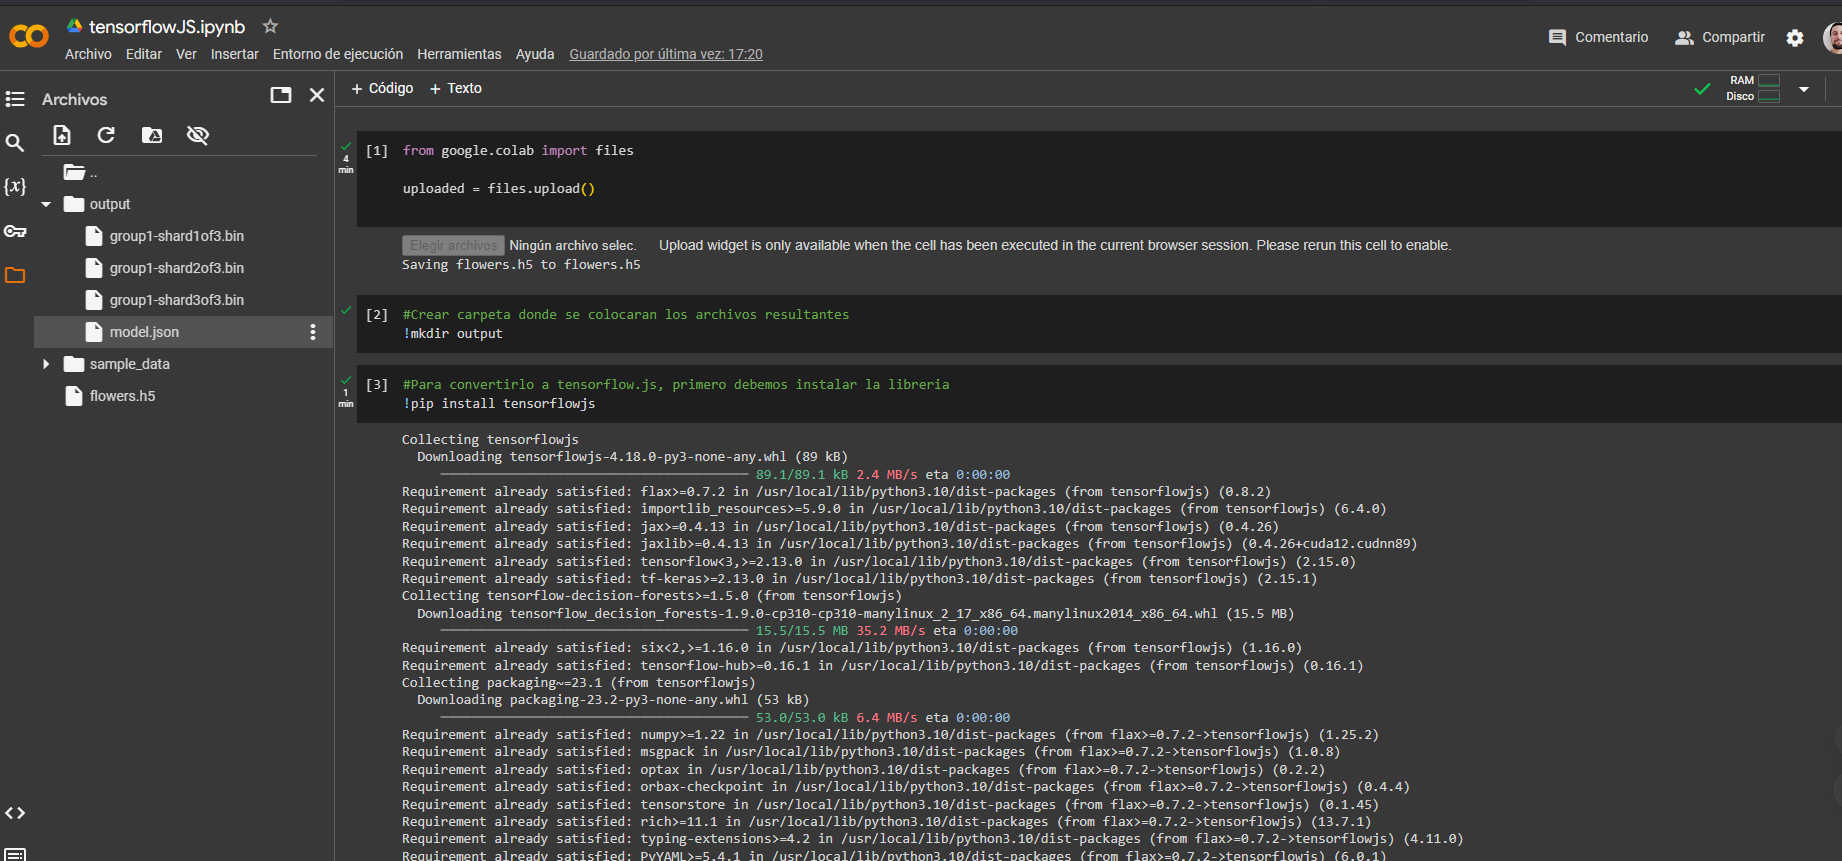
\includegraphics{Flores/img/Generar Json.png}
\caption{image.png}
\end{figure}

    Descargamos los archivos de la carpeta output y los añadimos a la
carpeta en donde se encuentra el html donde mostraremos el
funcionamiento del modelo con la camara del movil conectado al
ordenador.

    Abrimos el servidor en la carpeta donde tenemos guardado la pagina web

    \begin{figure}
\centering
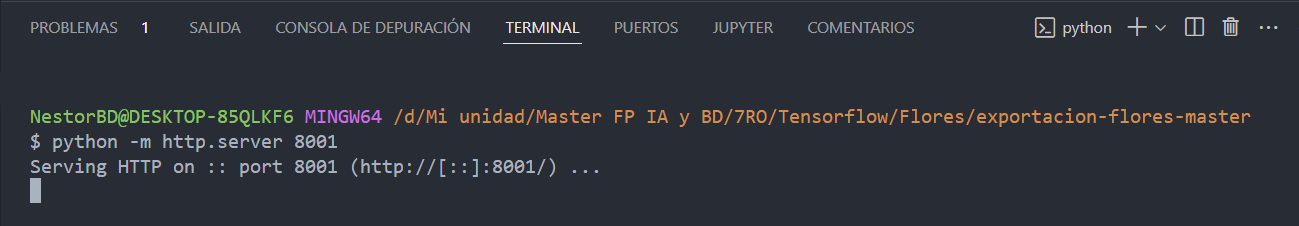
\includegraphics{Flores/img/Abrir servidor.png}
\caption{image.png}
\end{figure}

    Y por ultimo abrimos el \href{http://localhost:8001}{link} en donde
hemos alojado la web

    \begin{figure}
\centering
\includegraphics{Flores/img/Visualización en la web.png}
\caption{image.png}
\end{figure}

    \begin{figure}
\centering
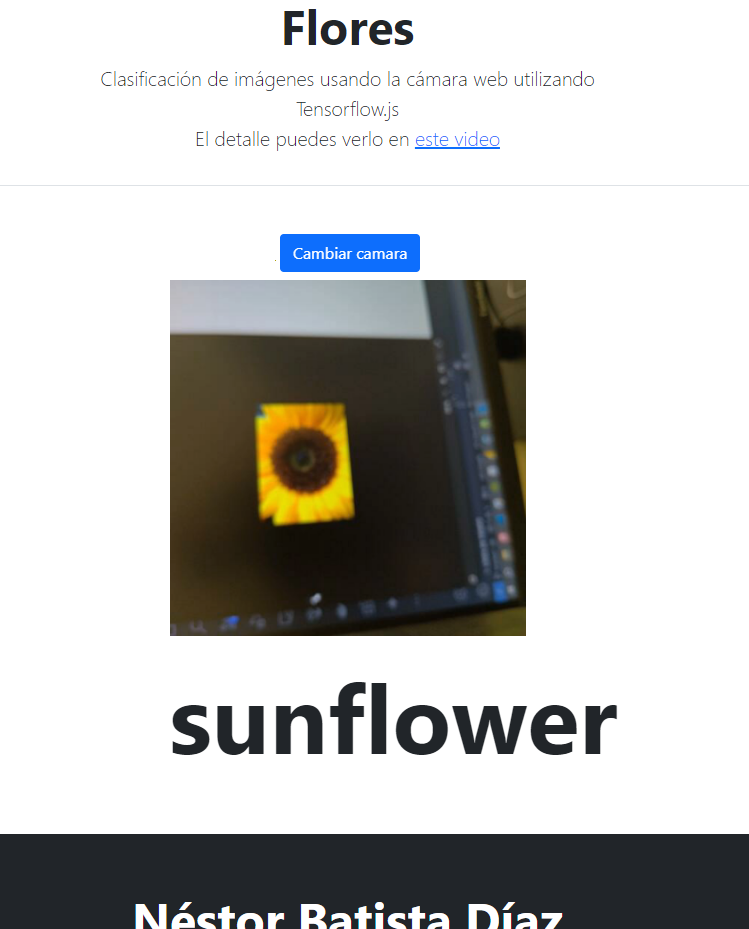
\includegraphics{Flores/img/sunflower.png}
\caption{image.png}
\end{figure}


    % Add a bibliography block to the postdoc
    
    
    
\end{document}
